% ============================================================
%  Shared preamble - matches the Mode-0 / Mode-1 report house style
% ============================================================
\documentclass[11pt,a4paper]{article}

\usepackage[utf8]{inputenc}
\usepackage[expansion=false]{microtype}
\usepackage[a4paper,left=28mm,right=28mm,top=28mm,bottom=25mm]{geometry}

\usepackage{amsmath,amssymb}
\usepackage{booktabs}
\usepackage{array}
\usepackage{enumitem}
\usepackage{xcolor}
\usepackage{caption}
\usepackage{fancyhdr}
\usepackage{titlesec}
\usepackage{tikz}
\usetikzlibrary{positioning,arrows.meta,calc,fit,backgrounds,shapes.geometric}
\usepackage[most]{tcolorbox}
\usepackage[section]{placeins}
\usepackage[hidelinks]{hyperref}

% ---------- colours ----------
\definecolor{navy}{RGB}{26,60,102}
\definecolor{accent}{RGB}{40,92,148}
\definecolor{softblue}{RGB}{232,240,248}
\definecolor{rulegrey}{RGB}{120,130,140}
\definecolor{orangeacc}{RGB}{196,106,48}
\definecolor{boxblue}{RGB}{219,232,244}
\definecolor{tealbox}{RGB}{214,236,238}
\definecolor{peachbox}{RGB}{250,226,208}
\definecolor{greybox}{RGB}{238,240,242}
\definecolor{greenbox}{RGB}{214,238,214}
\definecolor{pinkbox}{RGB}{250,216,224}

\hypersetup{
  colorlinks=true,
  linkcolor=accent,
  urlcolor=accent,
  citecolor=accent,
  pdftitle={Bluetooth Channel Sounding Mode-2 Phase-Based Ranging},
  pdfsubject={Formal technical report},
}

% ---------- headings ----------
\titleformat{\section}{\normalfont\Large\bfseries\color{navy}}{\thesection}{0.8em}{}
\titleformat{\subsection}{\normalfont\large\bfseries\color{navy}}{\thesubsection}{0.7em}{}
\titleformat{\subsubsection}{\normalfont\normalsize\bfseries\color{navy}}{\thesubsubsection}{0.6em}{}
\titlespacing*{\section}{0pt}{1.9\baselineskip}{0.8\baselineskip}
\titlespacing*{\subsection}{0pt}{1.2\baselineskip}{0.5\baselineskip}

% ---------- captions ----------
\captionsetup{font=small,labelfont={bf,color=accent},labelsep=colon,width=0.92\textwidth}
\captionsetup[table]{position=above,skip=4pt}
\captionsetup[figure]{position=below,skip=8pt}

% ---------- headers ----------
\pagestyle{fancy}
\fancyhf{}
\renewcommand{\headrulewidth}{0.6pt}
\fancyhead[L]{\small Bluetooth CS Mode-2 Phase-Based Ranging}
\fancyhead[R]{\small Formal technical report - Revision 1.0}
\fancyfoot[C]{\small\thepage}

% ---------- callout box ----------
\newtcolorbox{callout}[1][]{
  colback=softblue, colframe=accent, boxrule=0.5pt,
  left=6pt,right=6pt,top=5pt,bottom=5pt, arc=1pt,
  fontupper=\small, #1}

% ---------- normative reference box ----------
\newtcolorbox{specref}[1][]{
  colback=greybox, colframe=rulegrey, boxrule=0.5pt,
  left=6pt,right=6pt,top=4pt,bottom=4pt, arc=1pt,
  fontupper=\small, #1}

% ---------- table helpers ----------
\newcolumntype{L}[1]{>{\raggedright\arraybackslash}p{#1}}
\renewcommand{\arraystretch}{1.18}

% ---------- macros ----------
\newcommand{\us}{\,\ensuremath{\upmu}s}
\newcommand{\PCT}{\mathrm{PCT}}
\newcommand{\FFO}{\mathrm{FFO}}
\newcommand{\FAE}{\mathrm{FAE}}
\newcommand{\ToF}{\mathrm{ToF}}
\newcommand{\RTT}{\mathrm{RTT}}
\newcommand{\TQI}{\mathrm{TQI}}
\newcommand{\NADM}{\mathrm{NADM}}
\newcommand{\Tsw}{T_{SW}}
\newcommand{\Tpm}{T_{PM}}
\newcommand{\Trd}{T_{RD}}
\newcommand{\Tipp}{T_{IP2}}
\newcommand{\Nap}{N_{AP}}
\newcommand{\code}[1]{\texttt{\small #1}}
\providecommand{\upmu}{\mu}

% Core specification citation shorthand
\newcommand{\core}[1]{\textcolor{rulegrey}{\small[Core 6.3, #1]}}

% TikZ block styles reused across figures
\tikzset{
  blk/.style   ={draw=navy!70, fill=softblue, rounded corners=1pt, align=center,
                 font=\scriptsize, inner sep=3.5pt, minimum height=8mm},
  pblk/.style  ={draw=navy!70, fill=white, rounded corners=1pt, align=center,
                 font=\scriptsize, inner sep=3.5pt, minimum height=8mm},
  ar/.style    ={-{Latex[length=2mm]}, draw=navy!80, thick},
  dar/.style   ={-{Latex[length=2mm]}, draw=orangeacc, dashed, thin},
  slot/.style  ={draw=navy!55, font=\scriptsize, align=center, minimum height=7mm},
}

% ============================================================
\begin{document}

% ---------------- Title page ----------------
\thispagestyle{empty}
\vspace*{18mm}
{\color{accent}\small\bfseries FORMAL TECHNICAL REPORT \hfill REVISION 1.0}

\vspace{26mm}
{\raggedright\color{navy}\Huge\bfseries Bluetooth Channel Sounding\par}
\vspace{5mm}
{\raggedright\color{navy}\huge\bfseries Mode-2 Phase-Based Ranging\par}

\vspace{7mm}
\noindent{\raggedright\color{rulegrey}\large Tone exchange, the phase correction term, two-way
phase cancellation, phase-slope and impulse-response range estimation, and ambiguity resolution\par}

\vspace{12mm}
\noindent\rule{\textwidth}{1pt}

\vspace{4mm}
\noindent
This report traces the complete measurement chain of a Bluetooth Channel Sounding Mode-2 step: the
reciprocal exchange of unmodulated tones across $\Nap+1$ tone slots, the complex phase measurement
made in each slot, its reporting as a phase correction term, and the conversion of a set of
per-channel phase correction terms into a distance. It derives the two-way phase construction that
cancels the unknown relative local-oscillator phase, shows why that construction leaves the four
hardware phase responses as an additive loop group delay, and shows why a residual fractional
frequency offset from Mode-0 turns directly into a range bias through the interval between the two
measurements. It develops the estimator family that serves the observable: single-tone phase and
frequency estimation, weighted phase-slope regression, inverse-transform channel impulse response
formation, and super-resolution first-path detection, together with the Cram\'er--Rao analysis that
ties ranging variance to phase variance, channel count and frequency span. It closes with
ambiguity resolution against Mode-1, an error budget, a layered verification plan, and the boundary
between specified behaviour and implementation choice.

\vfill
\noindent
\begin{tabular}{@{}L{40mm}L{95mm}@{}}
Primary references & Core 6.3, Vol.\ 6, Part H, Sec.\ 4.3.3; Vol.\ 1, Part A, Sec.\ 9.2 \\
Air-interface timing & Core 6.3, Vol.\ 6, Part H, Secs.\ 4.3 and 4.5 \\
Host interface & Core 6.3, Vol.\ 4, Part E, LE CS Subevent Result event \\
Companion reports & \emph{Bluetooth CS Mode-0 Frequency Estimation}, Revision 4.0;
                    \emph{Bluetooth CS Mode-1 RTT Estimation}, Revision 1.0 \\
Document type & Scientific and implementation-oriented technical report \\
Revision date & 4 September 2026 \\
\end{tabular}

\newpage
\pagenumbering{roman}

% ---------------- Abstract ----------------
\section*{Abstract}
\addcontentsline{toc}{section}{Abstract}

Mode-2 is the phase-based ranging step of Bluetooth Low Energy Channel Sounding
\core{Vol.\ 6, Part H, Sec.\ 4.3.3}. The initiator transmits a sequence of unmodulated tones on the
step's channel, one per antenna path, and the reflector measures the complex amplitude of each; after
the interlude period $\Tipp$ the roles reverse and the initiator measures the reflector's tones. Each
device reports, per antenna path, a complex phase correction term. The sum of the two measured phases
removes the unknown relative local-oscillator phase and leaves twice the propagation phase. Repeating
this across the hopped channel set gives phase as a function of frequency, whose slope is the
round-trip delay and hence the distance.

The specification defines the tone-slot structure, the permitted timings, the antenna path
configuration and permutation, the reported phase correction term and tone quality indicator, and the
requirement that Mode-0 precede the ranging steps \core{Vol.\ 6, Part H, Secs.\ 4.3--4.5; Vol.\ 4,
Part E}. It does not mandate how phase is estimated from samples, how the per-channel terms are
combined, or how ambiguity is resolved: Volume 1, Part A, Section 9.2 describes distance estimation
from phase and amplitude information architecturally rather than normatively. This report therefore
separates normative behaviour from receiver and algorithm design.

It derives the two-way phase relation from oscillator-referenced phases, shows that the four
transmit and receive chain phase responses accumulate into a single additive loop group delay that
must be calibrated rather than assumed to cancel, and shows that a residual fractional frequency
offset $\epsilon$ produces a range bias $c\,\epsilon\,\Delta T/2$ set by the separation $\Delta T$
between the reciprocal measurements. A dedicated section develops the phase-estimator family and the
two families of range extraction --- slope regression in the frequency domain and peak search in the
inverse-transform domain --- with their ambiguity, resolution and multipath properties. A worked
example at 2\,440\,MHz over 72 channels quantifies the achievable ranging uncertainty, the cost of an
uncorrected clock scale error, and the reporting quantum. The report closes with an error budget, a
layered verification plan, and the specified/implementation boundary.

\begin{callout}
\textbf{Status and interpretation.} Normative claims are tied to the cited Bluetooth Core
Specification sections. Phase estimators, ranging algorithms, quality metrics, calibration databases
and aggregation rules are representative implementation methods. Timing parameter value lists,
antenna configuration indices and report field encodings should be read from the adopted
specification revision in force; where this report states them, they are given to make the equations
concrete, and section numbering within Volume 6, Part H has changed between Core revisions. The
Bluetooth specification and adopted test specifications remain authoritative for conformance.
\end{callout}

\newpage
\tableofcontents
\newpage
\pagenumbering{arabic}
\setcounter{page}{1}

% ============================================================
\section{Scope and measurement objective}
% ============================================================

Bluetooth Channel Sounding uses four step modes, defined in Core 6.3, Volume 6, Part H,
Sections 4.3.1--4.3.4. Mode-0 establishes the relative frequency and timing scale between the two
devices. Mode-1 uses that scale to measure a round-trip time. Mode-2 measures phase on tone
exchanges. Mode-3 combines a Mode-1 packet exchange with a Mode-2 tone exchange in a single step.

The Mode-2 measurement objective is not a distance and not a phase in radians. It is, per step and
per antenna path, a \emph{complex number} --- the phase correction term $\PCT$ --- expressed in the
measuring device's own local-oscillator reference, together with a tone quality indicator and enough
metadata to associate it with a channel and a physical antenna path
\core{Vol.\ 4, Part E, LE CS Subevent Result}. The engineering chain is

\begin{enumerate}[leftmargin=1.6em,itemsep=1pt]
  \item open the receive window on the step's channel at the expected carrier derived from the
        Mode-0 result, and capture each tone slot;
  \item estimate the complex amplitude of the tone in each slot, referenced to the local oscillator;
  \item map slot index to physical antenna path through the antenna path permutation, and report
        $\PCT$ and the tone quality indicator;
  \item at the ranging entity, form the two-way phase sum per channel and antenna path, which
        cancels the unknown relative oscillator phase;
  \item remove the calibrated loop phase response and the residual frequency-offset term;
  \item assemble the per-channel complex values into a frequency-domain channel estimate, and
        extract a delay by slope regression or by inverse transform with first-path detection; and
  \item resolve the periodic ambiguity of the phase observable against the Mode-1 round-trip-time
        estimate, and aggregate.
\end{enumerate}

\subsection{What Mode-2 measures and what it does not}

Mode-2 produces a \emph{precise} but \emph{ambiguous} distance estimate --- the exact complement of
Mode-1. Its precision follows from the synthesised aperture: measuring phase at $K$ channels spread
over a span $S$ of up to 74\,MHz gives a delay resolution of order $1/S \approx 13.5$\,ns, and a
thermal precision far below that, because a phase slope fitted through many high-signal-to-noise
points is located to a small fraction of one fringe. Its ambiguity follows from the same
periodicity: phase is known only modulo $2\pi$, so the distance repeats every $c/(2\Delta f)$, which
is 149.9\,m at the 1\,MHz channel spacing of the Bluetooth Low Energy channel raster.

\begin{callout}
\textbf{The CS channel raster is not contiguous, and the gap matters.} Channel Sounding uses 72 RF
channels at $2402+k$\,MHz for $k = 2\ldots22$ and $k = 26\ldots76$
\core{Vol.\ 6, Part A, Sec.\ 2}. They therefore run from 2404 to 2478\,MHz --- a span of
\emph{74}\,MHz, not 71 --- and there is a $4$\,MHz gap between 2424 and 2428\,MHz where channels
23, 24 and 25 are absent. The span sets the resolution and enters the precision bound; the largest
gap sets the limit beyond which sequential phase unwrapping fails, and $4$\,MHz is four times the
raster spacing. Section~\ref{sec:slope} returns to this: it reduces the safe unwrapping range from
$74.95$\,m to $18.74$\,m even before any channel is excluded by the channel map.
\end{callout}

\begin{callout}
\textbf{Three properties that are frequently confused.} (1) The two-way phase construction cancels the
unknown \emph{relative oscillator phase} of the two devices, but it \emph{accumulates} the four
transmit and receive chain phase responses --- exactly as the Mode-1 reciprocal construction cancels
the reflector turnaround but accumulates the four chain group delays. (2) A residual fractional
frequency offset does not merely add noise: because the residual offset in hertz scales with the
channel frequency, it produces a phase term \emph{linear in frequency}, which is indistinguishable
from range. (3) Multipath error in Mode-2 is \emph{not} one-sided. The phase slope of a superposition
is an amplitude-weighted quantity that can be biased short as easily as long, which is why
first-path detection in the transform domain matters more here than a robust combiner does.
\end{callout}

\subsection{Why the observable is reported, not the range}

The controller reports $\PCT$ values; it does not report a distance. Core 6.3, Volume 1, Part A,
Section 9.2 describes distance estimation from phase and amplitude information as an architectural
capability, and the mapping from a set of phase correction terms to a metre value is deliberately
left outside the specification. This is the single most important structural fact about Mode-2 for an
implementer: the entire accuracy-determining part of the chain --- phase estimation, calibration,
transform, first-path detection, ambiguity resolution, aggregation --- is design freedom, and
therefore is where accuracy is won or lost.

% ============================================================
\section{Normative framework and terminology}
% ============================================================

\begin{table}[h]
\caption{Normative map for the Mode-2 phase-based ranging measurement. Section numbering should be
confirmed against the specification revision in force.}
\label{tab:normmap}
\centering\small
\begin{tabular}{@{}L{42mm}L{51mm}L{51mm}@{}}
\toprule
Source & What it defines & Question answered \\
\midrule
Core 6.3, Vol.\ 1, Part A, Sec.\ 9.1 & CS procedure architecture; ordering of calibration and ranging steps & Why must Mode-0 precede Mode-2? \\
Core 6.3, Vol.\ 1, Part A, Sec.\ 9.2 & Distance estimation based on phase and amplitude information & What is the intended use of the reported phase? \\
Core 6.3, Vol.\ 6, Part H, Sec.\ 4.3.3 & Mode-2 step structure: tone slots, ordering, antenna paths & What is transmitted, in which order, and when? \\
Core 6.3, Vol.\ 6, Part H, Sec.\ 4.3 & $\Tsw$, $\Tpm$, $\Trd$, $\Tipp$, $T_{FCS}$ and permitted value sets & Which step timings may be configured? \\
Core 6.3, Vol.\ 6, Part H, Sec.\ 4.5 & Antenna path handling, permutation, tone extension slot & Which physical path does a slot correspond to? \\
Core 6.3, Vol.\ 6, Part A, Sec.\ 3.5 & Frequency measurement and generation in CS; expected frequencies for non-Mode-0 transmissions & On what carrier is the Mode-2 tone expected? \\
Core 6.3, Vol.\ 6, Part H, Sec.\ 4.2 & CS channel selection and hopping within a procedure & Which channels form the aperture, and in what order? \\
Core 6.3, Vol.\ 4, Part E, LE CS Subevent Result event & Per-step $\PCT$ and tone quality reporting & How is the measurement exposed to the host? \\
Core 6.3, Vol.\ 4, Part E, HCI CS configuration commands & Antenna configuration index, $\Tipp$, $\Tpm$, $\Tsw$, mode selection & How is the step parameterised? \\
RFPHY.TS / LL.TS, CS step Mode-2 clauses & Instrument-level verification of tone timing and phase reporting & How is the behaviour tested? \\
\bottomrule
\end{tabular}
\end{table}

\begin{table}[h]
\caption{Principal symbols.}
\label{tab:symbols}
\centering\small
\begin{tabular}{@{}L{28mm}L{78mm}L{22mm}@{}}
\toprule
Symbol & Meaning & Units \\
\midrule
$f_k$ & Carrier frequency of CS channel $k$ & Hz \\
$\Delta f$ & Channel spacing of the CS raster (1\,MHz) & Hz \\
$S$ & Frequency span actually measured, $f_{max}-f_{min}$ & Hz \\
$K$ & Number of channels contributing to one range estimate & --- \\
$\tau$ & One-way propagation delay, $d/c$ & s \\
$\theta_R(f_k)$ & Phase measured at the reflector on channel $k$ & rad \\
$\theta_I(f_k)$ & Phase measured at the initiator on channel $k$ & rad \\
$\Theta(f_k)$ & Two-way phase sum $\theta_I+\theta_R$ & rad \\
$\phi_I,\ \phi_R$ & Local-oscillator phases of the two devices & rad \\
$\PCT$ & Reported phase correction term, complex & --- \\
$H[k]$ & Assembled frequency-domain channel estimate & --- \\
$h(t)$ & Inverse-transform channel impulse response & --- \\
$\tau_\ell,\ a_\ell$ & Delay and complex gain of multipath component $\ell$ & s, --- \\
$D_{loop}$ & Total calibrated loop group delay of the four chains & s \\
$\Phi_{loop}(f)$ & Total calibrated loop phase response & rad \\
$\epsilon$ & Residual fractional frequency offset after Mode-0 & --- \\
$\Delta T$ & Interval between the reciprocal measurements of one path & s \\
$\Tsw$ & Antenna path switch period & s \\
$\Tpm$ & Phase measurement period & s \\
$\Trd$ & Transmitter ramp-down period & s \\
$\Tipp$ & Interlude period between initiator and reflector tone sequences & s \\
$\Nap$ & Number of antenna paths & --- \\
$\TQI$ & Tone quality indicator & index \\
\bottomrule
\end{tabular}
\end{table}
% ============================================================
\section{Position of Mode-2 in the CS subevent}
% ============================================================

Figure~\ref{fig:stack} places Mode-2 in the causal chain. Mode-0 runs first and produces the
subevent frequency reference $\FFO^{*}_{RX}$ \core{Vol.\ 6, Part H, Sec.\ 4.3.1}. That reference is
used for two distinct purposes in Mode-2: it places the expected carrier so the tone is received
close to the centre of the measurement filter, and it bounds the residual frequency offset whose
product with the reciprocal measurement interval is a direct range bias.

\begin{figure}[h]
\centering
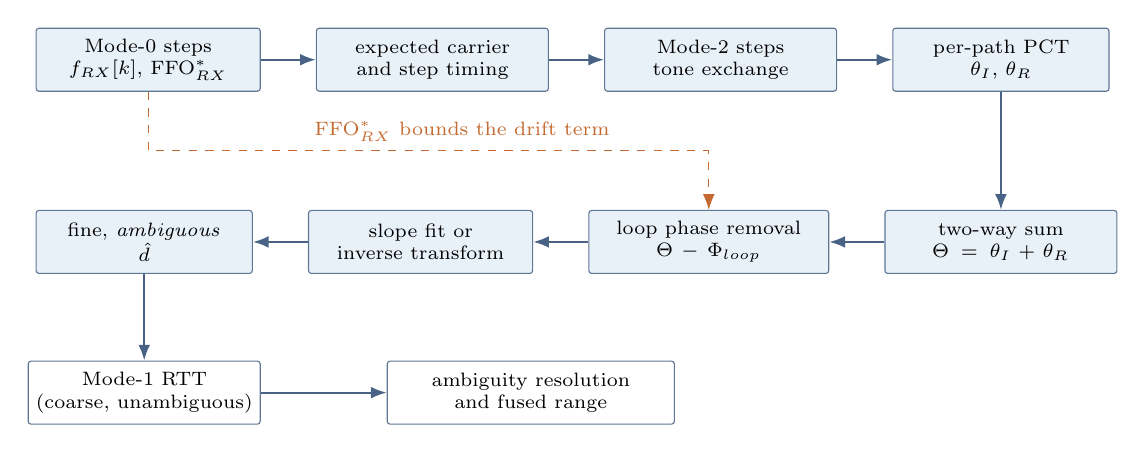
\begin{tikzpicture}[node distance=6mm and 7mm]
\node[blk,text width=26mm] (m0) {Mode-0 steps\\ $f_{RX}[k]$, $\FFO^{*}_{RX}$};
\node[blk,right=of m0,text width=27mm] (carr) {expected carrier\\ and step timing};
\node[blk,right=of carr,text width=27mm] (m2) {Mode-2 steps\\ tone exchange};
\node[blk,right=of m2,text width=25mm] (pct) {per-path $\PCT$\\ $\theta_I$, $\theta_R$};

\node[blk,below=15mm of pct,text width=27mm] (sum) {two-way sum\\ $\Theta=\theta_I+\theta_R$};
\node[blk,left=of sum,text width=28mm] (cal) {loop phase removal\\ $\Theta-\Phi_{loop}$};
\node[blk,left=of cal,text width=26mm] (fit) {slope fit or\\ inverse transform};
\node[blk,left=of fit,text width=25mm] (fine) {fine, \emph{ambiguous}\\ $\hat d$};

\node[pblk,below=11mm of fine,text width=27mm] (m1) {Mode-1 RTT\\ (coarse, unambiguous)};
\node[pblk,right=16mm of m1,text width=34mm] (fuse) {ambiguity resolution\\ and fused range};

\draw[ar] (m0)--(carr); \draw[ar] (carr)--(m2); \draw[ar] (m2)--(pct);
\draw[ar] (pct)--(sum); \draw[ar] (sum)--(cal); \draw[ar] (cal)--(fit); \draw[ar] (fit)--(fine);
\draw[ar] (fine)--(m1.north-|fine);
\draw[ar] (m1)--(fuse);
\draw[dar] (m0.south) |- ($(cal.north)+(0,7.5mm)$)
   node[pos=0.78,above,font=\scriptsize,color=orangeacc] {$\FFO^{*}_{RX}$ bounds the drift term}
   -- (cal.north);
\end{tikzpicture}
\caption{Position of Mode-2. Mode-0 supplies both the expected carrier and the bound on the residual
frequency offset that enters the two-way phase. Mode-2 produces a precise but periodic range which is
disambiguated by the Mode-1 estimate.}
\label{fig:stack}
\end{figure}

\subsection{Why Mode-2 cannot precede Mode-0}

Three independent effects make the ordering mandatory rather than conventional, and each is stronger
than the corresponding Mode-1 effect.

\emph{Carrier placement.} The phase measurement is made over a window of $\Tpm$, typically
10\us. A residual carrier offset $\delta f$ rotates the tone by $2\pi\,\delta f\,\Tpm$ within the
window. An uncorrected 12\,ppm crystal pair at 2.44\,GHz gives $\delta f = 29.3$\,kHz and therefore
$1.84$ rad of rotation \emph{inside a single measurement}, which destroys a naive coherent phase
estimate outright. Mode-0 exists so that the residual is small enough for the tone to be treated as
stationary in phase over $\Tpm$, or at worst as a small known linear ramp.

\emph{Reciprocal interval drift.} The reflector measures the initiator's tone at one instant and the
initiator measures the reflector's tone about $\Delta T$ later. Any residual frequency difference
accumulates $2\pi\,\delta f\,\Delta T$ of relative oscillator phase in between, and that term does
\emph{not} cancel in the two-way sum. Section~\ref{sec:freqerr} shows that because $\delta f$ scales
with the channel frequency, this term is linear in frequency and therefore reads directly as
distance: $c\,\epsilon\,\Delta T/2$, which is 34\,cm for an uncorrected 12\,ppm pair and
$\Delta T = 190$\us.

\emph{Frequency raster.} The tone must be generated at the channel's nominal centre as seen by the
peer \core{Vol.\ 6, Part A, Sec.\ 3.5}. A device that has not measured the peer's frequency error
places its tone at a frequency the peer does not expect, which biases the measurement by the
frequency-dependent part of the receive chain response and, in a narrow measurement filter, by
filter phase slope as well.

% ============================================================
\section{Mode-2 timing and the tone-slot structure}
\label{sec:timing}
% ============================================================

\subsection{One complete Mode-2 step}

Figure~\ref{fig:m2timing} shows the air-interface order of a Mode-2 step
\core{Vol.\ 6, Part H, Sec.\ 4.3.3}. Widths are labelled rather than drawn to scale, because the
tone-sequence duration depends on the antenna configuration and on the configured $\Tsw$ and $\Tpm$,
and $\Tipp$ is configured.

\begin{figure}[h]
\centering
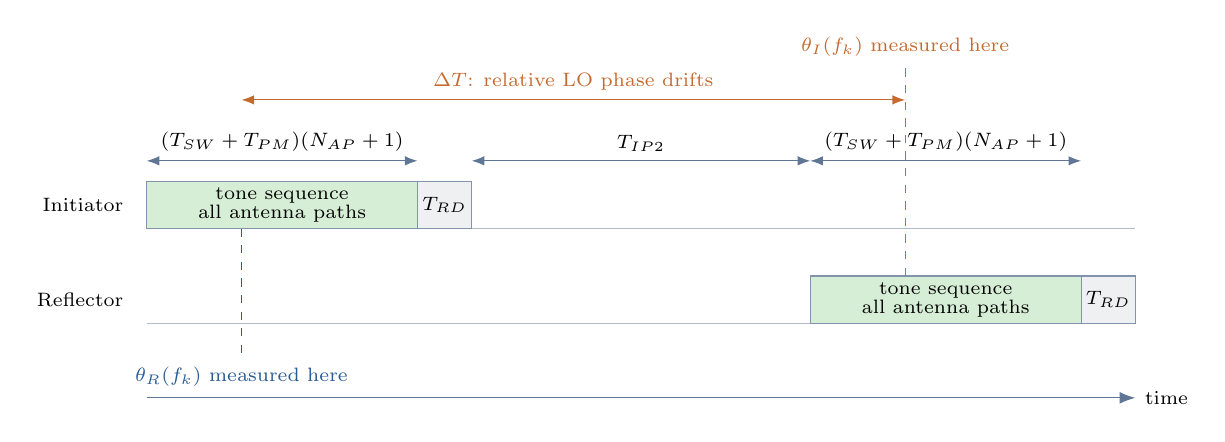
\begin{tikzpicture}[x=0.86mm,y=0.86mm]
\def\yI{14} \def\yR{0}
\draw[-{Latex[length=2mm]},draw=navy!70] (0,\yR-11) -- (146,\yR-11) node[right,font=\scriptsize] {time};
\node[font=\scriptsize,anchor=east] at (-2,\yI+3.5) {Initiator};
\node[font=\scriptsize,anchor=east] at (-2,\yR+3.5) {Reflector};
\draw[draw=navy!35] (0,\yI) -- (146,\yI);
\draw[draw=navy!35] (0,\yR) -- (146,\yR);

% initiator tone sequence
\draw[slot,fill=greenbox] (0,\yI) rectangle (40,\yI+7)
   node[midway,align=center] {tone sequence\\[-1pt] all antenna paths};
\draw[slot,fill=greybox] (40,\yI) rectangle (48,\yI+7) node[midway] {$\Trd$};

% reflector tone sequence
\draw[slot,fill=greenbox] (98,\yR) rectangle (138,\yR+7)
   node[midway,align=center] {tone sequence\\[-1pt] all antenna paths};
\draw[slot,fill=greybox] (138,\yR) rectangle (146,\yR+7) node[midway] {$\Trd$};

% brackets
\draw[{Latex[length=1.6mm]}-{Latex[length=1.6mm]},draw=navy!70] (0,\yI+10) -- (40,\yI+10)
   node[midway,above,font=\scriptsize] {$(\Tsw+\Tpm)(\Nap+1)$};
\draw[{Latex[length=1.6mm]}-{Latex[length=1.6mm]},draw=navy!70] (48,\yI+10) -- (98,\yI+10)
   node[midway,above,font=\scriptsize] {$\Tipp$};
\draw[{Latex[length=1.6mm]}-{Latex[length=1.6mm]},draw=navy!70] (98,\yI+10) -- (138,\yI+10)
   node[midway,above,font=\scriptsize] {$(\Tsw+\Tpm)(\Nap+1)$};

% measurement instants
\draw[dashed,draw=accent] (14,\yI) -- (14,\yR-5);
\node[font=\scriptsize,color=accent,anchor=north] at (14,\yR-5) {$\theta_R(f_k)$ measured here};
\draw[dashed,draw=orangeacc] (112,\yR+7) -- (112,\yI+24);
\node[font=\scriptsize,color=orangeacc,anchor=south] at (112,\yI+24) {$\theta_I(f_k)$ measured here};
\draw[{Latex[length=1.6mm]}-{Latex[length=1.6mm]},draw=orangeacc] (14,\yI+19) -- (112,\yI+19)
   node[midway,above,font=\scriptsize,color=orangeacc] {$\Delta T$: relative LO phase drifts};
\end{tikzpicture}
\caption{Mode-2 step. The initiator transmits a tone sequence covering every antenna path, ramps
down, and after the interlude period $\Tipp$ the reflector transmits its own tone sequence on the
same channel. Each device measures the phase of the tone it receives against its own local
oscillator. The interval $\Delta T$ between the two measurements of a given antenna path is the
interval over which the relative oscillator phase is free to drift.}
\label{fig:m2timing}
\end{figure}

The nominal step duration is
\begin{equation}
T_{step,2} \;=\; 2\bigl[(\Tsw+\Tpm)(\Nap+1) + \Trd\bigr] \;+\; \Tipp ,
\label{eq:stepdur}
\end{equation}
with the frequency-change period $T_{FCS}$ inserted between scheduled steps when consecutive steps
use different channels \core{Vol.\ 6, Part H, Sec.\ 4.3}. Note the structural difference from
Mode-1: there is no packet, so there is no $T_{SY}$; the transmission is a continuous unmodulated
carrier, and the step length is set by the number of antenna paths rather than by a sequence length.

The interval that matters for the frequency-error term is not $T_{step,2}$ but the separation
between the two measurements of the \emph{same} antenna path,
\begin{equation}
\Delta T \;=\; (\Tsw+\Tpm)(\Nap+1) \;+\; \Trd \;+\; \Tipp ,
\label{eq:deltaT}
\end{equation}
which for identical slot ordering in both directions is independent of which path is considered.

\subsection{The tone sequence and one tone slot}

Each tone sequence consists of $\Nap+1$ slots. Each slot is a switch period $\Tsw$, during which the
antenna switch changes state and the radio settles, followed by a phase measurement period $\Tpm$
during which a continuous unmodulated tone at the channel centre frequency is transmitted and the
peer makes its measurement \core{Vol.\ 6, Part H, Secs.\ 4.3.3 and 4.5}.

\begin{figure}[h]
\centering
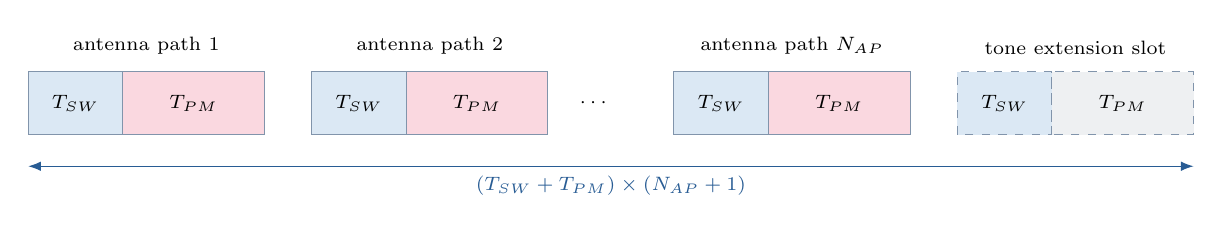
\begin{tikzpicture}[x=1mm,y=1mm]
% slots
\foreach \i/\x in {1/0, 2/36}{
  \draw[slot,fill=boxblue] (\x,0) rectangle (\x+12,8) node[midway] {$\Tsw$};
  \draw[slot,fill=pinkbox] (\x+12,0) rectangle (\x+30,8) node[midway] {$\Tpm$};
  \node[font=\scriptsize,anchor=south] at (\x+15,9) {antenna path \i};
}
\node[font=\scriptsize] at (72,4) {$\cdots$};
\draw[slot,fill=boxblue] (82,0) rectangle (94,8) node[midway] {$\Tsw$};
\draw[slot,fill=pinkbox] (94,0) rectangle (112,8) node[midway] {$\Tpm$};
\node[font=\scriptsize,anchor=south] at (97,9) {antenna path $\Nap$};
\draw[slot,fill=boxblue,dashed] (118,0) rectangle (130,8) node[midway] {$\Tsw$};
\draw[slot,fill=greybox,dashed] (130,0) rectangle (148,8) node[midway] {$\Tpm$};
\node[font=\scriptsize,anchor=south,align=center] at (133,9) {tone extension slot};

\draw[{Latex[length=1.6mm]}-{Latex[length=1.6mm]},draw=accent] (0,-4) -- (148,-4)
  node[midway,below,font=\scriptsize,color=accent] {$(\Tsw+\Tpm)\times(\Nap+1)$};
\end{tikzpicture}
\caption{Tone sequence structure within one transmit slot. The first $\Nap$ slots carry the tone on
successive antenna paths; the final slot is the tone extension slot, whose transmission is
configurable and whose reception gives a same-step estimate of the noise and interference floor.}
\label{fig:tonesequence}
\end{figure}

\begin{table}[h]
\caption{Mode-2 step timing parameters. Permitted sets are configuration-dependent and are subject to
both devices' declared capabilities; read the value lists from the specification revision in force
\core{Vol.\ 6, Part H, Sec.\ 4.3; Vol.\ 4, Part E, CS configuration}.}
\label{tab:timing}
\centering\small
\begin{tabular}{@{}L{18mm}L{54mm}L{56mm}@{}}
\toprule
Parameter & Meaning & Representative permitted values \\
\midrule
$\Tsw$    & Antenna path switch period, including RF and phase settling & 1, 2, 4, 10\us when switching is performed; 0 with a single antenna \\
$\Tpm$    & Phase measurement period & 10, 20, 40\us ($40\us$ mandatory) \\
$\Trd$    & Transmitter ramp-down & 5\us \\
$\Tipp$   & Interlude period, end of initiator ramp-down to start of reflector tone sequence & 10, 20, 30, 40, 50, 60, 80, 145\us \\
$T_{FCS}$ & Frequency-change period between steps & 15, 20, 30, 40, 50, 60, 80, 100, 120, 150\us \\
\bottomrule
\end{tabular}
\end{table}

\begin{callout}
\textbf{$\Tsw$ is not dead time.} The switch period exists so that the antenna switch, any tuning
network and the receive chain reach a settled state before the measurement window opens. Two
implementation consequences follow. First, the local oscillator must run \emph{continuously} across
the whole tone sequence: if it is retuned, restarted or re-locked between slots, the antenna paths
no longer share a common phase reference and the per-path terms cannot be compared. Second, $\Tsw$
must be chosen against the measured settling time of the actual switch and filter, not against the
minimum permitted value; residual settling inside $\Tpm$ appears as a slot-dependent phase bias that
looks exactly like an antenna calibration error.
\end{callout}

\subsection{Step durations for representative configurations}

\begin{table}[h]
\caption{Tone-sequence and step durations from Eqs.~\eqref{eq:stepdur} and~\eqref{eq:deltaT}, with
$\Trd = 5\us$ and $\Tipp = 145\us$.}
\label{tab:durations}
\centering\small
\begin{tabular}{@{}rrrrrr@{}}
\toprule
$\Nap$ & $\Tsw$ & $\Tpm$ & Tone sequence & $T_{step,2}$ & $\Delta T$ \\
\midrule
1 & $10\us$ & $10\us$ & $40\us$  & $235\us$ & $190\us$ \\
1 & $2\us$  & $10\us$ & $24\us$  & $203\us$ & $174\us$ \\
2 & $2\us$  & $10\us$ & $36\us$  & $227\us$ & $186\us$ \\
4 & $2\us$  & $10\us$ & $60\us$  & $275\us$ & $210\us$ \\
4 & $10\us$ & $20\us$ & $150\us$ & $455\us$ & $300\us$ \\
4 & $2\us$  & $10\us$ & $60\us$  & $140\us$ ($\Tipp=10\us$) & $75\us$ \\
\bottomrule
\end{tabular}
\end{table}

Table~\ref{tab:durations} gives the tone-sequence duration, the step duration and the reciprocal
measurement interval for representative parameter sets. Its last two rows carry the design message
of this section: they differ only in $\Tipp$ and $\Tpm$, yet their $\Delta T$ values differ by a
factor of four. Every microsecond added to $\Delta T$
multiplies the residual frequency error into range through Eq.~\eqref{eq:epsbias}. A configuration
chosen for antenna coverage and phase averaging is simultaneously a configuration that relaxes or
tightens the Mode-0 accuracy requirement by a factor of four.

% ============================================================
\section{Antenna paths, permutation, and the tone extension slot}
\label{sec:antenna}
% ============================================================

\subsection{Antenna configuration}

The number of antenna paths is not chosen directly; it follows from the antenna configuration index
agreed for the procedure, which states how many antenna elements each side contributes
\core{Vol.\ 6, Part H, Sec.\ 4.5; Vol.\ 4, Part E, CS configuration}. Each path is one
(initiator element, reflector element) pair, and every path is measured in both directions within
the step.

\begin{table}[h]
\caption{Antenna configuration index and the resulting number of antenna paths, per
\core{Vol.\ 6, Part A, Sec.\ 5.3}. Device A is the initiator and device B the reflector; $\Nap$ is
bounded to $1 \le \Nap \le 4$.}
\label{tab:aci}
\centering\small
\begin{tabular}{@{}cccc@{\hspace{10mm}}cccc@{}}
\toprule
ACI & Initiator & Reflector & $\Nap$ & ACI & Initiator & Reflector & $\Nap$ \\
\midrule
0 & 1 & 1 & 1 & 4 & 1 & 2 & 2 \\
1 & 2 & 1 & 2 & 5 & 1 & 3 & 3 \\
2 & 3 & 1 & 3 & 6 & 1 & 4 & 4 \\
3 & 4 & 1 & 4 & 7 & 2 & 2 & 4 \\
\bottomrule
\end{tabular}
\end{table}

\subsection{Antenna path permutation}

The order in which antenna paths occupy the tone slots is not fixed across steps. An antenna path
permutation index is applied per step and is reported alongside the measurement, so that the ranging
entity can map slot index back to physical path \core{Vol.\ 6, Part H, Sec.\ 4.5; Vol.\ 4, Part E,
LE CS Subevent Result}. Permuting the order decorrelates any slot-position-dependent bias --- switch
settling, thermal transients, oscillator pulling from the preceding slot --- from the physical path,
so that such biases average across steps instead of accumulating into a per-path offset.

\begin{callout}
\textbf{A permutation error is silent and fatal.} If the ranging entity applies the wrong permutation,
it attributes each channel's phase to the wrong antenna path. The per-path phase-versus-frequency
sequences then interleave contributions from physically different paths with different geometric
delays, and the slope fit returns a plausible-looking number that is simply wrong. There is no
internal consistency check that catches this in a single-path geometry, so it must be verified
explicitly against a known asymmetric antenna layout.
\end{callout}

\subsection{The tone extension slot}

The final slot of each sequence is the tone extension slot. Whether it is actually transmitted is
configurable, and the receiving device reports whether a tone was present
\core{Vol.\ 6, Part H, Sec.\ 4.3.3; Vol.\ 4, Part E}. It serves two purposes that are worth
separating.

\begin{itemize}[leftmargin=1.4em,itemsep=1pt]
  \item \textbf{In-step noise and interference floor.} A slot in which the peer is known not to
    transmit gives a measurement of everything that is not the tone, taken on the same channel, with
    the same gain state, microseconds away from the signal measurement. That is a far better noise
    reference than any out-of-step estimate, and it is the natural denominator for a per-tone
    signal-to-noise estimate and hence for the tone quality indicator.
  \item \textbf{Asymmetric capability handling.} A device that needs additional settling or that
    supports fewer paths can use the extension slot to keep the two sequences aligned in duration,
    which keeps $\Delta T$ common to both directions.
\end{itemize}

An implementation that discards the extension slot measurement is discarding the only same-step,
same-channel, same-gain noise reference the step provides.

\subsection{Multiple paths as independent observables}

With $\Nap>1$, one step yields $\Nap$ two-way phase values on the same channel. They are not
redundant: the paths have different geometric lengths, different antenna phase centres and
different multipath realisations. Three uses are common, and they are different algorithms rather
than variations of one.

\begin{enumerate}[leftmargin=1.6em,itemsep=1pt]
  \item \textbf{Diversity.} Select or weight paths by tone quality to reject a path that is in a
    deep fade on that channel. This is the most robust use and the cheapest.
  \item \textbf{Averaging.} Combine per-path range estimates after removing the per-path antenna
    offsets from the calibration table. This reduces variance but is only valid once the offsets are
    known to better than the precision being claimed.
  \item \textbf{Angle information.} The phase differences \emph{between} paths on one channel carry
    the direction of arrival, exactly as in a conventional array. This is outside the ranging chain
    but shares the calibration.
\end{enumerate}
% ============================================================
\section{From two tones to a two-way phase}
\label{sec:twoway}
% ============================================================

\subsection{Oscillator-referenced phases}

Let the two devices run local oscillators whose phases at time $t$ on channel $k$ are
\begin{equation}
\varphi_I(t) \;=\; 2\pi f_k t + \phi_I ,
\qquad
\varphi_R(t) \;=\; 2\pi f_k (1+\epsilon) t + \phi_R ,
\label{eq:los}
\end{equation}
where $\epsilon$ is the residual fractional frequency offset that survives the Mode-0 correction and
$\phi_I,\phi_R$ are unknown constants. Set $\epsilon=0$ for the moment; Section~\ref{sec:freqerr}
restores it.

The initiator transmits its tone during the slot for antenna path $p$; the reflector receives it
after the propagation delay $\tau$ and measures the phase of the received tone against its own
oscillator. Ignoring hardware for the moment,
\begin{equation}
\theta_R(f_k) \;=\; -2\pi f_k \tau \;+\; (\phi_I - \phi_R) .
\label{eq:thetaR}
\end{equation}
After $\Delta T$ the roles reverse and the initiator measures
\begin{equation}
\theta_I(f_k) \;=\; -2\pi f_k \tau \;+\; (\phi_R - \phi_I) .
\label{eq:thetaI}
\end{equation}

\subsection{The cancellation}

Adding Eqs.~\eqref{eq:thetaR} and~\eqref{eq:thetaI},
\begin{equation}
\Theta(f_k) \;\equiv\; \theta_I(f_k) + \theta_R(f_k) \;=\; -4\pi f_k \tau ,
\label{eq:twoway}
\end{equation}
and the unknown relative oscillator phase has cancelled exactly. This is the phase-domain analogue of
the Mode-1 reciprocal timestamp construction: neither device needs to know the other's oscillator
phase, only what it measured against its own.

\begin{figure}[h]
\centering
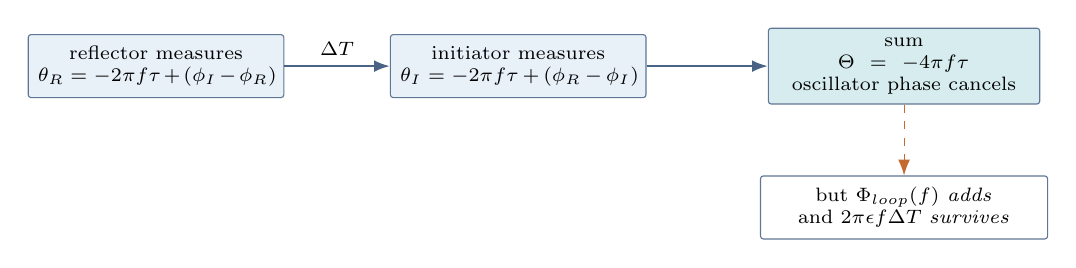
\begin{tikzpicture}[x=1mm,y=1mm,font=\scriptsize]
\node[blk,text width=30mm] (a) at (0,0) {reflector measures\\ $\theta_R=-2\pi f\tau+(\phi_I-\phi_R)$};
\node[blk,text width=30mm] (b) at (46,0) {initiator measures\\ $\theta_I=-2\pi f\tau+(\phi_R-\phi_I)$};
\node[blk,text width=32mm,fill=tealbox] (c) at (95,0) {sum\\ $\Theta=-4\pi f\tau$\\ oscillator phase cancels};
\draw[ar] (a)--(b) node[midway,above,font=\scriptsize] {$\Delta T$};
\draw[ar] (b)--(c);
\node[pblk,text width=34mm,below=9mm of c] (d) {but $\Phi_{loop}(f)$ \emph{adds}\\ and $2\pi\epsilon f\Delta T$ \emph{survives}};
\draw[dar] (c)--(d);
\end{tikzpicture}
\caption{The two-way phase construction. The unknown relative oscillator phase cancels in the sum;
the hardware phase responses and the residual-frequency drift term do not.}
\label{fig:cancel}
\end{figure}

\subsection{Hardware phase responses accumulate}
\label{sec:loopphase}

Devices do not measure phase at the antenna. Each measurement includes the transmit-chain phase
response of the transmitting device and the receive-chain phase response of the measuring device.
Writing $\Phi_{TX,X}(f)$ and $\Phi_{RX,X}(f)$ for device $X$,
\begin{align}
\theta_R(f_k) &= -2\pi f_k\tau + (\phi_I-\phi_R) - \Phi_{TX,I}(f_k) - \Phi_{RX,R}(f_k), \\
\theta_I(f_k) &= -2\pi f_k\tau + (\phi_R-\phi_I) - \Phi_{TX,R}(f_k) - \Phi_{RX,I}(f_k),
\end{align}
so that
\begin{equation}
\Theta(f_k) \;=\; -4\pi f_k \tau \;-\;
  \underbrace{\bigl[\Phi_{TX,I}+\Phi_{RX,R}+\Phi_{TX,R}+\Phi_{RX,I}\bigr](f_k)}_{\textstyle \Phi_{loop}(f_k)} .
\label{eq:loopphase}
\end{equation}
To the extent that $\Phi_{loop}$ is linear in frequency it is a pure delay,
$\Phi_{loop}(f) \approx \Phi_0 + 2\pi f D_{loop}$, and it is then indistinguishable from range:
\begin{equation}
\hat d_{biased} \;=\; d \;+\; \frac{c\,D_{loop}}{2} .
\label{eq:loopbias}
\end{equation}

\begin{callout}
\textbf{The same result as Mode-1, reached by a different route.} Equation~\eqref{eq:loopbias} is
numerically identical to the Mode-1 loop-delay bias: an uncalibrated $D_{loop}$ of 10\,ns produces
$1.50$\,m of range error, independent of true distance and of signal-to-noise ratio, and no amount
of averaging removes it. The difference is that Mode-2 is sensitive to the \emph{whole shape} of
$\Phi_{loop}(f)$, not only to its slope: any curvature --- from filter roll-off at the band edges,
from a VCO tuning-dependent phase, from an antenna's own phase response --- appears as a
frequency-dependent residual that corrupts the slope fit and smears the inverse transform. A Mode-2
calibration is therefore a \emph{phase response over frequency}, per antenna path and per gain state,
not the single scalar that suffices for Mode-1.
\end{callout}

The practical form of the correction is
\begin{equation}
\Theta_{cal}(f_k) \;=\; \mathrm{wrap}\bigl(\Theta(f_k) + \hat\Phi_{loop}(f_k)\bigr),
\label{eq:phasecal}
\end{equation}
applied before any unwrapping, with $\hat\Phi_{loop}$ read from a calibration surface indexed by
channel, antenna path, gain state and temperature. The constant term $\Phi_0$ affects the intercept
rather than the slope, and is therefore harmless to a slope estimator but not to an
inverse-transform estimator, which sees it as a complex rotation of the impulse response.

\subsection{Residual frequency offset: the term that reads as distance}
\label{sec:freqerr}

Restoring $\epsilon$ in Eq.~\eqref{eq:los}, the relative oscillator phase is no longer constant
between the two measurements. Over the interval $\Delta T$ of Eq.~\eqref{eq:deltaT} it advances by
$2\pi \epsilon f_k \Delta T$, and this term appears in the sum with a single sign:
\begin{equation}
\Theta(f_k) \;=\; -4\pi f_k \tau \;-\; \Phi_{loop}(f_k) \;+\; 2\pi \epsilon f_k \Delta T .
\label{eq:epsterm}
\end{equation}
Because $\epsilon$ is a \emph{fractional} offset, the term is proportional to $f_k$. It is therefore
linear in frequency, exactly like the propagation term, and a slope estimator cannot separate the
two. Differentiating and converting to distance,
\begin{equation}
\delta d_\epsilon \;=\; \frac{c\,\epsilon\,\Delta T}{2} .
\label{eq:epsbias}
\end{equation}

\begin{table}[h]
\caption{Range bias from residual fractional frequency offset, Eq.~\eqref{eq:epsbias}.}
\label{tab:epsbias}
\centering\small
\begin{tabular}{@{}lrrr@{}}
\toprule
Residual offset & $\Delta T=75\us$ & $\Delta T=190\us$ & $\Delta T=300\us$ \\
\midrule
$12$\,ppm (uncorrected, typical crystal pair) & $13.5$\,cm & $34.2$\,cm & $54.0$\,cm \\
$1$\,ppm (crude correction)   & $1.12$\,cm & $2.85$\,cm & $4.50$\,cm \\
$0.1$\,ppm                    & $1.12$\,mm & $2.85$\,mm & $4.50$\,mm \\
$0.05$\,ppm (good Mode-0 result) & $0.56$\,mm & $1.42$\,mm & $2.25$\,mm \\
\bottomrule
\end{tabular}
\end{table}

Three design conclusions follow, and they differ sharply from the Mode-1 case. First, the accuracy
Mode-0 must deliver for Mode-2 is roughly an order of magnitude more demanding than for Mode-1,
because Mode-2's own thermal floor is an order of magnitude lower: 1\,ppm is adequate for Mode-1 and
is already the dominant error for Mode-2. Second, a short $\Tipp$ and a compact tone sequence are
directly worth range accuracy. Third, the term is a \emph{bias common to every channel in the
subevent}, so averaging across channels does not reduce it --- only the Mode-0 correction does.

\subsection{Distance from the two-way phase}

Neglecting the corrected terms, Eq.~\eqref{eq:twoway} gives the fundamental relation
\begin{equation}
\Theta(f) \;=\; -\frac{4\pi f d}{c},
\qquad
d \;=\; -\frac{c}{4\pi}\,\frac{\partial \Theta}{\partial f} ,
\label{eq:dfromslope}
\end{equation}
and the two constants worth memorising are the phase step per channel and the ambiguity period:
\begin{equation}
\frac{\partial\Theta}{\partial f}\,\Delta f
  \;=\; \frac{4\pi\,\Delta f}{c}\,d
  \;=\; 0.041917\ \text{rad/m at }\Delta f = 1\,\text{MHz},
\qquad
d_{amb} \;=\; \frac{c}{2\Delta f} \;=\; 149.90\ \text{m}.
\label{eq:consts}
\end{equation}
Equivalently, one metre of distance advances the two-way phase by $2.402^{\circ}$ per megahertz of
channel separation, and the observable repeats every 149.90\,m. Unwrapping between \emph{adjacent}
channels is safe only while the step is below $\pi$, that is while
\begin{equation}
d \;<\; \frac{c}{4\Delta f_{max}} ,
\label{eq:unwraplimit}
\end{equation}
where $\Delta f_{max}$ is the \emph{largest} spacing between consecutive measured channels, not the
raster pitch. For adjacent 1\,MHz channels this is $74.95$\,m, but the CS raster's own $4$\,MHz gap
reduces it to $18.74$\,m, and any further exclusion by the channel
map reduces it again.

% ============================================================
\section{Signal-level model: tone to complex amplitude}
\label{sec:signal}
% ============================================================

\subsection{Received tone}

During $\Tpm$ the peer transmits an unmodulated carrier. Over a multipath channel with $L$
components,
\begin{equation}
r(t) \;=\; \Re\left\{ \sum_{\ell=1}^{L} a_\ell\,
   e^{\,j\left(2\pi f_k (t-\tau_\ell) + \phi_{tx}\right)} \right\} + n(t),
\label{eq:rxtone}
\end{equation}
with $\tau_1 \le \cdots \le \tau_L$ so that $\tau_1$ is the first-arriving path. After quadrature
downconversion against the local oscillator and sampling,
\begin{equation}
z[n] \;=\; A\,e^{\,j(2\pi \delta f\, n T_s + \theta)} \;+\; w[n],
\qquad n = 0,\dots,N-1,\quad N = \Tpm/T_s,
\label{eq:zn}
\end{equation}
where the complex amplitude $A e^{j\theta}$ is the \emph{sum over paths}
\begin{equation}
A e^{\,j\theta} \;=\; \sum_{\ell=1}^{L} a_\ell\, e^{-j 2\pi f_k \tau_\ell} \;=\; H(f_k),
\label{eq:Hfk}
\end{equation}
$\delta f$ is the residual carrier offset left after Mode-0, and $w[n]$ is complex noise of variance
$\sigma_w^2$ per sample.

Equation~\eqref{eq:Hfk} is the central identity of Mode-2 and deserves to be stated plainly: the
quantity measured in one tone slot on one channel is one frequency-domain sample of the channel
transfer function. Everything downstream is the reconstruction of a channel response from a set of
such samples.

\subsection{The estimation problem}

\begin{callout}
\textbf{Problem statement.} Given samples $z[n]$ from one tone slot, estimate the complex amplitude
$Ae^{j\theta}$ of the tone in the presence of an unknown small residual frequency offset $\delta f$,
receiver DC offset, and I/Q imbalance; report it as a phase correction term together with a quality
indicator. Then, given the set $\{\Theta(f_k)\}$ over channels, estimate the delay $\tau_1$ of the
first-arriving component and convert it to a distance.
\end{callout}

The problem splits cleanly into a per-slot estimation problem and a cross-channel estimation problem,
and the two have entirely different characters. The per-slot problem is a classical single-tone
parameter estimation with an excellent signal-to-noise ratio and a very short record. The
cross-channel problem is a spectral-estimation problem on non-uniformly sampled, wrapped, hopped
data. Most implementations lose more accuracy in the second than in the first.

% ============================================================
\section{Per-slot phase estimators}
\label{sec:phaseest}
% ============================================================

None of this section is mandated by the specification; all of it is constrained by it, in that the
tone is unmodulated, the observation length is $\Tpm$, the carrier is fixed by the channel and the
reporting format is fixed by the host interface.

\subsection{Coherent average and the DFT bin}
\label{sec:coh}

The maximum-likelihood estimate of $Ae^{j\theta}$ for known $\delta f$ is the coherent average after
derotation:
\begin{equation}
\widehat{Ae^{j\theta}} \;=\; \frac{1}{N}\sum_{n=0}^{N-1} z[n]\, e^{-j2\pi \delta f\, n T_s},
\qquad
\hat\theta = \arg\Bigl(\widehat{Ae^{j\theta}}\Bigr).
\label{eq:cohavg}
\end{equation}
With $\delta f$ unknown, evaluating Eq.~\eqref{eq:cohavg} on a grid of candidate offsets is exactly a
discrete Fourier transform of the slot, and the estimate is taken at the maximum-magnitude bin. Zero
padding refines the frequency grid; the phase must be read at the refined maximum, not at the nearest
coarse bin, because a half-bin frequency error rotates the phase by up to $\pi$ across the record.

\paragraph{Coherent loss.} An uncorrected offset $\delta f$ attenuates the coherent sum by
$|\mathrm{sinc}(\delta f\,\Tpm)|$ and, more importantly, biases the phase by
$\pi\,\delta f\,\Tpm$ --- half the total rotation, since the average sits at the record centre. At
$\Tpm = 10\us$, a 1\,kHz residual gives $0.0157$ rad of phase bias. This is the mechanism that
converts a Mode-0 error into a Mode-2 error \emph{within} a slot, distinct from the
$\Delta T$ mechanism of Section~\ref{sec:freqerr}, and it is largely common-mode between the two
directions and therefore partially cancels in the sum.

\subsection{Frequency estimation before phase}

Because the phase estimate is only as good as the derotation, a well-designed slot estimator
estimates $\delta f$ first. Three standard estimators apply directly.

\paragraph{Kay's estimator.} A weighted average of successive phase increments,
\begin{equation}
\widehat{\delta f} \;=\; \frac{1}{2\pi T_s}\sum_{n=1}^{N-1} u_n\,
   \arg\bigl(z[n]z^{*}[n-1]\bigr),
\qquad
u_n \propto n(N-n),
\label{eq:kay}
\end{equation}
which attains the Cram\'er--Rao bound at high signal-to-noise ratio and costs one pass.

\paragraph{Fitz / Luise--Reggiannini.} Average the autocorrelation over several lags and take the
phase of the weighted sum; more robust than Eq.~\eqref{eq:kay} at moderate signal-to-noise ratio, at
the cost of a bounded acquisition range set by the maximum lag.

\paragraph{Rife--Boorstyn.} Coarse DFT peak followed by a local Newton refinement of the periodogram;
this is the maximum-likelihood estimator for a single tone in white noise and is the natural
reference implementation.

\begin{callout}
\textbf{Do not estimate $\delta f$ independently in every slot.} The residual offset is a property of
the oscillator pair over the subevent, not of the slot. Estimating it per slot adds an independent
noisy quantity to each phase estimate --- and, since the derotation bias is
$\pi\,\widehat{\delta f}\,\Tpm$, injects $\pi\Tpm\,\sigma_{\delta f}$ of extra phase noise per slot.
Estimate it jointly across the slots of a step, or carry it from Mode-0, and use the per-slot
estimate only as a consistency check.
\end{callout}

\subsection{Front-end impairments}

Three impairments bias a tone phase measurement in ways that a modulated-packet receiver largely
escapes, because a tone sits at a single frequency and does not average them out.

\paragraph{DC offset.} A receiver DC offset adds a constant to $z[n]$ and therefore a vector to the
coherent average. If the tone is placed at exactly zero intermediate frequency, the offset is
indistinguishable from the tone. Two standard mitigations are to place the tone at a deliberate
non-zero intermediate frequency so that the DC term falls in a different DFT bin, and to measure the
offset in the tone extension slot and subtract it. The first is strongly preferable.

\paragraph{I/Q imbalance.} Gain and phase mismatch between the in-phase and quadrature paths creates
an image at $-\delta f$. Its interference with the wanted tone produces a phase error that depends on
$\delta f$ and on the image rejection ratio; at 30\,dB of image rejection the worst-case phase error
is about $\arcsin(10^{-1.5}) = 1.8^{\circ}$, which is $0.031$ rad --- comparable to the entire
thermal phase budget of Section~\ref{sec:crlb}. Image rejection is therefore a ranging specification,
not only a sensitivity specification, and residual imbalance should be calibrated per gain state.

\paragraph{Phase noise.} Oscillator phase noise integrated over $\Tpm$ adds directly to $\theta$.
Unlike thermal noise it is correlated between the slots of one sequence, so it does not average down
across antenna paths within a step, though it does average across steps on different channels.

\subsection{Quality metrics and the tone quality indicator}

The per-slot estimator should emit, alongside $\PCT$, at least: the estimated tone amplitude, the
residual power after subtracting the fitted tone, the extension-slot noise reference, the estimated
$\delta f$ and its deviation from the subevent value, and any gain-change or clipping flag. The tone
quality indicator reported to the host is a small ordinal summary of these
\core{Vol.\ 4, Part E, LE CS Subevent Result}; the mapping is an implementation characterisation.

\begin{table}[h]
\caption{Reported tone quality indicator scale. The mapping from receiver metrics onto these levels
is an implementation characterisation, not a specified formula.}
\label{tab:tqi}
\centering\small
\begin{tabular}{@{}cl@{\hspace{14mm}}cl@{}}
\toprule
Value & Interpretation & Value & Interpretation \\
\midrule
0x0 & Tone quality high   & 0x2 & Tone quality low \\
0x1 & Tone quality medium & 0x3 & Tone quality unavailable \\
\bottomrule
\end{tabular}
\end{table}
% ============================================================
\section{From per-channel phase to distance}
\label{sec:range}
% ============================================================

The ranging entity receives, for each measured channel $k$ and each antenna path $p$, the two
reported phase correction terms. It forms
\begin{equation}
H[k] \;=\; \PCT_I[k]\;\PCT_R[k] \;\;\Longrightarrow\;\;
\arg H[k] = \theta_I(f_k)+\theta_R(f_k) = \Theta(f_k),
\label{eq:formH}
\end{equation}
that is, the two-way phase is obtained by \emph{multiplying} the two complex terms rather than by
adding two unwrapped angles. This is not a stylistic preference: multiplication in the complex plane
is immune to the wrapping of the individual measurements, whereas adding two \code{atan2} outputs
requires each to be unwrapped first, which is impossible for an isolated channel.

Figure~\ref{fig:estchain} shows how the range estimators compose. As in Mode-1, a practical design is
a chain: a robust ambiguity-free stage, a precise ambiguous stage, and a bias-correcting stage.

\begin{figure}[h]
\centering
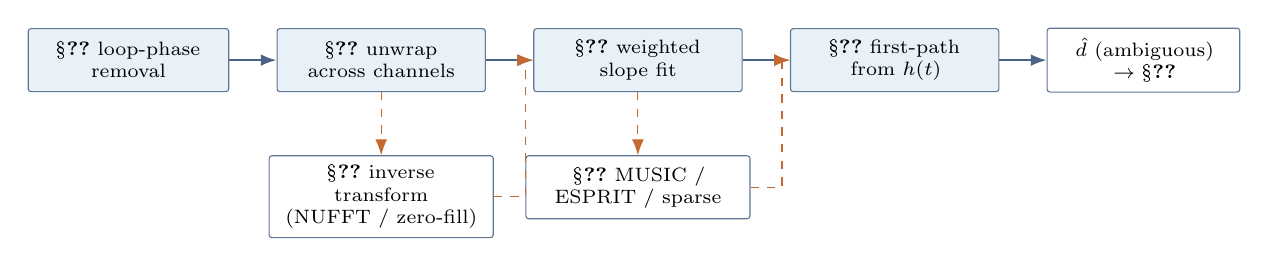
\begin{tikzpicture}[node distance=5mm and 6mm]
\node[blk,text width=23mm] (cal) {\S\ref{sec:loopphase} loop-phase\\ removal};
\node[blk,right=of cal,text width=24mm] (unw) {\S\ref{sec:slope} unwrap\\ across channels};
\node[blk,right=of unw,text width=24mm] (slope) {\S\ref{sec:slope} weighted\\ slope fit};
\node[blk,right=of slope,text width=24mm] (fp) {\S\ref{sec:ifft} first-path\\ from $h(t)$};
\node[pblk,below=8mm of unw,text width=26mm] (ifft) {\S\ref{sec:ifft} inverse transform\\ (NUFFT / zero-fill)};
\node[pblk,below=8mm of slope,text width=26mm] (sr) {\S\ref{sec:superres} MUSIC /\\ ESPRIT / sparse};
\node[pblk,right=of fp,text width=22mm] (out) {$\hat d$ (ambiguous)\\ $\to$ \S\ref{sec:fusion}};
\draw[ar] (cal)--(unw); \draw[ar] (unw)--(slope); \draw[ar] (slope)--(fp); \draw[ar] (fp)--(out);
\draw[dar] (unw)--(ifft); \draw[dar] (ifft.east) -- ++(4mm,0) |- (slope.west);
\draw[dar] (slope)--(sr); \draw[dar] (sr.east) -- ++(4mm,0) |- (fp.west);
\end{tikzpicture}
\caption{Range-estimator composition. Solid path: the common calibrate--unwrap--fit--correct chain.
Dashed: transform-domain and super-resolution alternatives that replace or augment a stage.}
\label{fig:estchain}
\end{figure}

% ------------------------------------------------------------
\subsection{Weighted phase-slope regression}
\label{sec:slope}

Order the measured channels by frequency --- they are visited in hopped order within the procedure
\core{Vol.\ 6, Part H, Sec.\ 4.2}, so the first operation is a sort, not a fit --- unwrap
$\Theta(f_k)$ across the sorted list, and fit a straight line weighted by tone quality:
\begin{equation}
\widehat{\frac{\partial\Theta}{\partial f}} \;=\;
\frac{\sum_k w_k (f_k-\bar f_w)(\Theta_k-\bar\Theta_w)}{\sum_k w_k (f_k-\bar f_w)^2},
\qquad
\hat d \;=\; -\frac{c}{4\pi}\,\widehat{\frac{\partial\Theta}{\partial f}},
\label{eq:slopefit}
\end{equation}
with $w_k$ derived from the per-tone signal-to-noise estimate, and $\bar f_w$, $\bar\Theta_w$ the
weighted means.

This is the exact frequency-domain dual of the Mode-1 group-delay regression: there the fit is over
the 2\,MHz of one packet, here it is over the full measured span. The estimators are identical; the
apertures differ by a factor of about forty, and that factor is precisely the ratio of their
resolutions and the reason one is unambiguous and the other is not.

\paragraph{Unwrapping is the fragile step.} Sequential unwrapping fails whenever the true
channel-to-channel phase step exceeds $\pi$, which by Eq.~\eqref{eq:unwraplimit} happens beyond
74.95\,m for adjacent 1\,MHz channels but only $18.74$\,m across the raster's built-in $4$\,MHz gap. It also fails on a single noisy or
faded channel, and a single unwrap error propagates as a step to \emph{all} subsequent channels,
producing a large and confident-looking range error. Three practical countermeasures:

\begin{itemize}[leftmargin=1.4em,itemsep=1pt]
  \item Seed the unwrap with the Mode-1 range, so that the predicted phase at each channel is known
    to within a small fraction of a fringe and unwrapping becomes a nearest-integer decision rather
    than a sequential accumulation.
  \item Weight or exclude low-quality tones before unwrapping, not after.
  \item Prefer a wrapped-domain estimator that never unwraps at all: maximise
    \[
      \Bigl|\;\sum_k w_k\, H[k]\; e^{\,j 4\pi f_k d/c}\;\Bigr|
    \]
    over a grid of $d$. This is the periodogram of the channel data in the delay domain, and it is
    exactly the inverse transform of Section~\ref{sec:ifft} evaluated on an arbitrarily fine grid.
\end{itemize}

\paragraph{Residual as a diagnostic.} The fit residual is as valuable as the slope. A residual that is
flat and consistent with the tone quality estimates indicates a clean single-path channel; a
systematically curved residual indicates uncorrected $\Phi_{loop}$ curvature; an oscillatory residual
with a period in frequency of $1/\Delta\tau$ is the unmistakable signature of a second path at delay
separation $\Delta\tau$ from the first.

% ------------------------------------------------------------
\subsection{Inverse transform and the channel impulse response}
\label{sec:ifft}

Because $H[k]$ is a set of frequency-domain samples of the channel (Eq.~\eqref{eq:Hfk}), an inverse
transform gives an estimate of the channel impulse response:
\begin{equation}
h(t) \;=\; \sum_k w_k\, H[k]\, e^{\,j 2\pi f_k t},
\qquad
\hat d \;=\; \frac{c\,\hat\tau_{2way}}{2},
\label{eq:cir}
\end{equation}
where $\hat\tau_{2way}$ is the delay of the first significant peak of $|h(t)|$.

The properties of Eq.~\eqref{eq:cir} follow directly from the sampling geometry:

\begin{table}[h]
\caption{Transform-domain properties for the full 72-channel CS raster ($S=74$\,MHz, 1\,MHz pitch, one 4\,MHz gap).}
\label{tab:transform}
\centering\small
\begin{tabular}{@{}L{50mm}L{40mm}L{40mm}@{}}
\toprule
Property & Expression & Value ($K=72$, $S=74$\,MHz) \\
\midrule
Delay resolution & $1/S$ & $13.5$\,ns \\
Range resolution & $c/(2S)$ & $2.03$\,m \\
Unambiguous delay span & $1/\Delta f$ & $1.00\us$ \\
Unambiguous range span & $c/(2\Delta f)$ & $149.90$\,m \\
Safe sequential-unwrap range & $c/(4\Delta f_{max})$ & $18.74$\,m (4\,MHz gap) \\
Sidelobe level, no window & $-13.3$\,dB & --- \\
Sidelobe level, Hann window & $-31.5$\,dB, $1.5\times$ wider main lobe & --- \\
\bottomrule
\end{tabular}
\end{table}

\paragraph{Non-uniform channel sets.} The CS channel list excludes some channels and the procedure may
not visit every remaining one in every subevent \core{Vol.\ 6, Part H, Sec.\ 4.2}. The resulting
non-uniform sampling makes a plain inverse fast Fourier transform inapplicable. Three remedies, in
increasing order of cost and fidelity: zero-fill the missing bins and accept the raised sidelobes;
interpolate the missing bins from the fitted model and accept the resulting bias toward that model;
or evaluate Eq.~\eqref{eq:cir} directly on a delay grid as a non-uniform transform, which is exact
and, for the few hundred delay bins of interest, entirely affordable.

\paragraph{Windowing is a bias--resolution trade.} An unwindowed transform has $-13.3$\,dB sidelobes,
so a strong reflector at $+30$\,ns can raise a sidelobe above a weak first path and capture the peak
search. A Hann window suppresses this at the cost of a 50\% wider main lobe, which \emph{increases}
the bias when two paths are genuinely unresolved. The correct choice depends on the channel and is
worth making adaptively, on the observed dynamic range of $|h(t)|$.

\paragraph{First-path detection.} Exactly as in Mode-1, the first peak matters and the largest peak
does not. Back-search thresholding and constant-false-alarm-rate leading-edge detection transfer
directly, with the threshold referenced to the sidelobe floor of the chosen window rather than to a
correlation sidelobe level.

\begin{callout}
\textbf{Slope fitting and transform peaks are not the same estimator.} A weighted slope fit returns
the amplitude-weighted mean delay of all the paths present; the transform peak search returns the
delay of a selected path. In a clean single-path channel they agree, and the slope fit is more
precise. In multipath they disagree, and the slope fit is \emph{wrong} in a way that no amount of
averaging repairs. A good implementation computes both and uses their disagreement as its multipath
indicator.
\end{callout}

% ------------------------------------------------------------
\subsection{Super-resolution methods}
\label{sec:superres}

Treating $H[k]$ as a uniformly sampled sum of complex exponentials in the frequency variable makes
the classical super-resolution machinery available: MUSIC and root-MUSIC on the covariance formed by
spatial smoothing over frequency sub-apertures, ESPRIT on the shift-invariance of the same
sub-apertures, and sparse recovery --- orthogonal matching pursuit or an $\ell_1$ formulation --- over
a dictionary of delay atoms.

These methods separate paths closer than $1/S$, which is where the $2.03$\,m resolution of
Table~\ref{tab:transform} becomes the limiting factor in an indoor room. They come with three
conditions that are frequently understated. They need an estimate of the model order, and they
degrade sharply when it is wrong. They need either multiple snapshots or spatial smoothing, and
smoothing spends aperture, so a 72-channel set smoothed into sub-apertures of 48 has an effective
resolution set by about 49\,MHz rather than 74\,MHz. And they are far more sensitive than a slope fit to
residual $\Phi_{loop}$ curvature, because a calibration error that a linear fit absorbs into its
intercept appears to a subspace method as an additional spurious component.

Unlike Mode-1, where super-resolution over a single 2\,MHz packet buys almost nothing, Mode-2 has
the aperture to make these methods genuinely useful. They are the natural home of the accuracy that
distinguishes a good phase-based implementation from an adequate one.

% ------------------------------------------------------------
\subsection{Comparison of range estimators}

\begin{table}[htb]
\caption{Range-estimator comparison for the Mode-2 observable.}
\label{tab:estcmp}
\centering\small
\begin{tabular}{@{}L{33mm}L{30mm}L{31mm}L{26mm}@{}}
\toprule
Method & Strength & Weakness & Typical role \\
\midrule
Weighted slope fit (\S\ref{sec:slope}) & Attains the bound in a clean channel; cheap & Needs unwrapping; multipath-biased & Default estimator \\
Wrapped-domain periodogram & No unwrapping; ambiguity explicit & Grid search cost & Robust alternative \\
Zero-filled inverse FFT (\S\ref{sec:ifft}) & Fast; shows the channel & Sidelobes from gaps & Diagnosis, first path \\
Non-uniform transform & Exact for any channel set & Cost scales with grid & Reference implementation \\
Windowed transform + CFAR & Robust first-path detection & Resolution loss from window & Multipath channels \\
MUSIC / root-MUSIC (\S\ref{sec:superres}) & Resolves below $1/S$ & Model order; smoothing cost & High-accuracy mode \\
ESPRIT & Closed-form, no search & Sensitive to calibration error & High-accuracy mode \\
Sparse recovery & Handles gaps naturally & Regularisation tuning & Post-processing \\
Mode-1-seeded unwrap (\S\ref{sec:fusion}) & Removes ambiguity entirely & Requires valid RTT & Always, where available \\
\bottomrule
\end{tabular}
\end{table}

% ============================================================
\section{Precision: the Cram\'er--Rao analysis}
\label{sec:crlb}
% ============================================================

\subsection{Phase precision in one tone slot}

For a single tone of energy $\mathcal{E}$ in white noise of one-sided density $N_0$, the phase
estimation variance is bounded by
\begin{equation}
\sigma_\theta \;\ge\; \frac{1}{\sqrt{2\,\mathcal{E}/N_0}},
\qquad
\frac{\mathcal{E}}{N_0} \;=\; \gamma\, B_n\, \Tpm ,
\label{eq:phasecrlb}
\end{equation}
where $\gamma$ is the signal-to-noise ratio measured in a reference noise bandwidth $B_n$. Taking
$B_n = 1$\,MHz and $\Tpm = 10\us$ gives a processing gain of exactly 10, so a 20\,dB in-band
signal-to-noise ratio yields $\mathcal{E}/N_0 = 30$\,dB and
$\sigma_\theta = 0.0224$\,rad $=1.28^{\circ}$.

The two-way phase is the sum of two independent measurements, so
\begin{equation}
\sigma_\Theta \;=\; \sqrt{\sigma_{\theta,I}^2 + \sigma_{\theta,R}^2} \;=\; \sqrt2\,\sigma_\theta
\quad\text{(symmetric links)} .
\label{eq:sigmaTheta}
\end{equation}

\subsection{Ranging precision from the slope fit}

For $K$ channels at frequencies $f_k$ with equal weights, the slope variance of the fit
Eq.~\eqref{eq:slopefit} is $\sigma_\Theta^2 / \sum_k (f_k-\bar f)^2$, so
\begin{equation}
\sigma_d \;=\; \frac{c}{4\pi}\,
   \frac{\sigma_\Theta}{\sqrt{\sum_k (f_k-\bar f)^2}}
   \;=\; \frac{c}{4\pi}\,\frac{\sqrt2\,\sigma_\theta}{S}\,
   \sqrt{\frac{12(K-1)}{K(K+1)}} ,
\label{eq:sigmad}
\end{equation}
the second form holding for $K$ channels spread uniformly over a span $S$. Three levers appear, and
only three: the frequency span $S$, the number of channels $K$, and the per-tone signal-to-noise
ratio through $\sigma_\theta$. Span is the strongest, entering linearly; channel count and
signal-to-noise ratio each enter as a square root.

\begin{table}[h]
\caption{Cram\'er--Rao ranging standard deviation from Eqs.~\eqref{eq:phasecrlb}--\eqref{eq:sigmad},
with $B_n = 1$\,MHz, evaluated on the actual CS channel raster. $\gamma$ is the per-tone in-band
signal-to-noise ratio; the unwrap limit is set by the largest gap in each subset, not by the pitch. These are bounds on the
\emph{random} error only; they say nothing about the calibration and multipath biases that dominate
Table~\ref{tab:example}.}
\label{tab:crlb}
\centering\small
\begin{tabular}{@{}rrrrrrr@{}}
\toprule
$\gamma$ & $\Tpm$ & $K$ & Span $S$ & $\sigma_\theta$ & Unwrap limit & $\sigma_d$ \\
\midrule
30\,dB & $10\us$ & 72 & 74\,MHz & $0.41^{\circ}$ & $18.74$\,m & $1.29$\,mm \\
20\,dB & $10\us$ & 72 & 74\,MHz & $1.28^{\circ}$ & $18.74$\,m & $4.07$\,mm \\
10\,dB & $10\us$ & 72 & 74\,MHz & $4.05^{\circ}$ & $18.74$\,m & $12.9$\,mm \\
 0\,dB & $10\us$ & 72 & 74\,MHz & $12.8^{\circ}$ & $18.74$\,m & $40.6$\,mm \\
20\,dB & $20\us$ & 72 & 74\,MHz & $0.91^{\circ}$ & $18.74$\,m & $2.87$\,mm \\
20\,dB & $40\us$ & 72 & 74\,MHz & $0.64^{\circ}$ & $18.74$\,m & $2.03$\,mm \\
20\,dB & $10\us$ & 36 & 73\,MHz & $1.28^{\circ}$ & $14.99$\,m & $5.74$\,mm \\
20\,dB & $10\us$ & 18 & 71\,MHz & $1.28^{\circ}$ & $10.71$\,m & $8.11$\,mm \\
10\,dB & $10\us$ & 18 & 71\,MHz & $4.05^{\circ}$ & $10.71$\,m & $25.7$\,mm \\
\bottomrule
\end{tabular}
\end{table}

\begin{callout}
\textbf{Reading Table~\ref{tab:crlb}.} Compare the 20\,dB, 72-channel row --- $4.3$\,mm --- with the
corresponding Mode-1 figure of $8.6$\,cm for 32 averaged steps at the same signal-to-noise ratio.
Phase-based ranging is roughly twenty times more precise for the same air time, and that is the
entire reason the mode exists. The comparison also shows where the effort must go: at a thermal floor
of a few millimetres, a $0.1$\,ns loop-delay calibration residual ($1.5$\,cm) and a $0.05$\,ppm
Mode-0 residual ($1.4$\,mm at $\Delta T = 190\us$) are no longer negligible corrections but the
leading terms. Note also the sixth and seventh rows: halving the channel count costs only
$\sqrt{2}$ in precision but halves the unwrap limit, which is an availability failure rather than an
accuracy one.
\end{callout}

% ============================================================
\section{Reference estimation procedure for one Mode-2 step}
% ============================================================

The following is a complete implementation path, not a mandated algorithm.

\begin{enumerate}[label=\textbf{P\arabic*.},leftmargin=2.6em,itemsep=2pt]
  \item Compute the expected carrier for this step from the Mode-0 subevent reference and the
    channel's nominal centre \core{Vol.\ 6, Part A, Sec.\ 3.5}; programme the local oscillator once
    for the whole tone sequence and do not retune, restart or re-lock it between slots.
  \item Derive the slot schedule from $\Tsw$, $\Tpm$, $\Nap$ and the step role; derive the antenna
    path permutation for this step and record it with the measurement.
  \item For each slot, open the measurement window strictly inside $\Tpm$, with a guard at both ends
    that covers switch settling and the peer's timing tolerance; capture $z[n]$ and record the gain
    state.
  \item Estimate the residual frequency offset jointly across the slots of the step, or apply the
    subevent value from Mode-0; do not re-estimate it independently per slot.
  \item Derotate and form the coherent average, Eq.~\eqref{eq:cohavg}; retain amplitude, phase, and
    the residual power after removing the fitted tone.
  \item Measure the tone extension slot with the same gain state and derive the noise and
    interference reference for this step.
  \item Compute the tone quality indicator from amplitude, residual and noise reference; mark a slot
    unavailable rather than reporting a low-confidence phase as if it were good.
  \item Scale and quantise the complex amplitude to the reported $\PCT$ format only at the interface
    boundary; retain full precision internally.
  \item Emit the record $\{$step, channel, role, antenna path permutation, per-path $\PCT$, per-path
    $\TQI$, extension-slot indication, gain state, estimated $\delta f$, flags$\}$
    \core{Vol.\ 4, Part E, LE CS Subevent Result}.
  \item At the ranging entity: pair the initiator and reflector terms per channel and path, form
    $H[k]$ by complex multiplication (Eq.~\eqref{eq:formH}), apply $\hat\Phi_{loop}$
    (Eq.~\eqref{eq:phasecal}) and the $\epsilon\Delta T$ correction (Eq.~\eqref{eq:epsterm}), sort by
    frequency, and run the estimator chain of Figure~\ref{fig:estchain}.
\end{enumerate}
% ============================================================
\section{Aggregation across steps, paths and subevents}
\label{sec:agg}
% ============================================================

\subsection{What is aggregated}

Mode-2 differs from Mode-1 in the level at which combination happens. A Mode-1 step yields a complete
range estimate that is then averaged. A Mode-2 step yields \emph{one frequency-domain sample} per
antenna path; the estimate exists only once the samples are assembled. Aggregation therefore has two
distinct layers.

\begin{enumerate}[leftmargin=1.6em,itemsep=1pt]
  \item \textbf{Within an assembly.} Channels measured within one coherent interval are combined
    \emph{coherently}, as the input to Eq.~\eqref{eq:slopefit} or~\eqref{eq:cir}. This is where the
    aperture --- and therefore the precision --- comes from, and it requires that the loop phase,
    the frequency offset and the geometry be stable across the whole set.
  \item \textbf{Across assemblies.} Successive subevents each yield a range estimate; these are
    combined \emph{incoherently}, by weighted mean, median or a tracking filter.
\end{enumerate}

\begin{callout}
\textbf{The coherence interval is a physical limit, not a configuration choice.} Coherent assembly is
valid only while the geometry is stable to a small fraction of a wavelength. At 2.44\,GHz the
wavelength is 12.3\,cm, so a tenth of a wavelength is 1.2\,cm; a relative velocity of $1$\,m/s covers
that in 12\,ms. A procedure whose channel sweep takes longer than the coherence interval must either
segment the sweep and combine the segments incoherently, or estimate and remove the range rate as
part of the fit --- which is a joint estimation of delay and Doppler, not a phase-slope fit.
\end{callout}

\subsection{Per-tone validity gating}

A tone should be gated out or heavily down-weighted when: the reported tone quality indicator is low
or unavailable in either direction; the tone amplitude is inconsistent with the extension-slot noise
reference; the residual after removing the fitted tone is large; the per-slot estimated $\delta f$
deviates from the subevent value; the gain state changed within $\Tpm$; clipping occurred; the
antenna path permutation could not be resolved; or the peer did not report a term for that channel
and path.

\subsection{Weighted combination and robust alternatives}

Within an assembly, weights enter the fit directly through $w_k$. Across assemblies, with $\hat d_m$
the estimate from assembly $m$ and $\sigma_m$ its predicted uncertainty,
\begin{equation}
w_m \;=\; g_m \min\!\left(w_{max},\ \frac{1}{\sigma_m^2+\sigma_{floor}^2}\right),
\qquad
\hat d \;=\; \frac{\sum_m w_m \hat d_m}{\sum_m w_m},
\label{eq:agg}
\end{equation}
with the floor $\sigma_{floor}$ representing the irreducible calibration and multipath contribution
and the cap $w_{max}$ preventing a single optimistic assembly from dominating.

Where the Mode-1 report recommends a lower-quantile combiner because multipath bias there is
one-sided and positive, that recommendation does \emph{not} transfer to Mode-2. A phase-slope
estimate under multipath is an amplitude-weighted mean delay and can be biased in either direction; a
transform-domain first-path estimate is biased long, like Mode-1, but only after it has correctly
identified a first path. The right robust statistic is therefore the median rather than a low
quantile, and the more valuable robustness comes from the multipath \emph{indicator} of
Section~\ref{sec:ifft} --- the disagreement between the slope fit and the transform peak --- used to
switch estimators rather than to trim samples.

% ============================================================
\section{Ambiguity resolution and the relationship to Mode-1 and Mode-3}
\label{sec:fusion}
% ============================================================

\subsection{The complementary pair}

\begin{table}[h]
\caption{Complementary character of the two ranging observables. The Mode-1 column reproduces the
companion report's figures for the same signal-to-noise ratio.}
\label{tab:fusion}
\centering\small
\begin{tabular}{@{}L{34mm}L{45mm}L{45mm}@{}}
\toprule
Property & Mode-1 (RTT) & Mode-2 (phase slope) \\
\midrule
Observable & Packet arrival time & Channel phase $\Theta(f)$ versus $f$ \\
Aperture & One packet, $\approx 2$\,MHz & Hopped band, up to $74$\,MHz \\
Resolution & $\approx 500$\,ns, $75$\,m & $\approx 13.5$\,ns, $2.03$\,m \\
Thermal precision at 20\,dB & $8.6$\,cm (32 steps) & $4.1$\,mm (72 channels) \\
Ambiguity & None over the operating range & Periodic, $149.90$\,m \\
Dominant error & Loop delay bias; thermal jitter & Loop phase response; Mode-0 residual; multipath \\
Multipath character & One-sided, biased long & Two-sided for slope; long for first path \\
Needs from Mode-0 & $\approx 1$\,ppm & $\approx 0.1$\,ppm \\
Integrity & Unpredictable waveform, $\NADM$ & None intrinsic; see \S\ref{sec:security} \\
\bottomrule
\end{tabular}
\end{table}

\subsection{How the ambiguity is actually resolved}

At the 1\,MHz Bluetooth Low Energy channel raster the phase observable repeats every 149.90\,m, which
any usable Mode-1 estimate clears by two orders of magnitude. Ambiguity resolution in the strict
sense --- choosing the correct fringe --- is therefore not the difficult part of Mode-2 in a standard
configuration. Two related problems are the difficult part, and they are frequently conflated with it.

\emph{Unwrap seeding.} Sequential unwrapping across channels fails on gaps and on faded tones long
before the 149.90\,m limit is approached, and each failure is a discrete range error. Seeding the
unwrap with the Mode-1 range converts a fragile sequential accumulation into $K$ independent
nearest-integer decisions, each of which is safe provided the Mode-1 uncertainty is well below
$c/(4 f_{gap})$ for the largest gap present. This is the operationally important use of Mode-1.

\emph{Path selection.} Choosing which peak of $|h(t)|$ is the direct path is a decision the phase
observable cannot make alone in a strongly reflective channel. Mode-1's estimate, being an
independent measurement with a different failure mode, bounds the search window.

\begin{callout}
\textbf{The fusion is hierarchical, not symmetric.} Mode-1 supplies a coarse, unambiguous,
attack-resistant scale; Mode-2 supplies precision within it. The correct architecture computes the
Mode-1 range first, uses it to seed unwrapping and to window the first-path search, and reports the
Mode-2 result with the Mode-1 result retained as a consistency check. A Mode-2 range that disagrees
with Mode-1 by more than the combined uncertainty is not a more precise answer; it is a detected
fault --- an unwrap slip, a permutation error, a wrong fringe, or an attack.
\end{callout}

\subsection{Mode-3}

Mode-3 performs a \code{CS\_SYNC} exchange and a tone exchange within a single step
\core{Vol.\ 6, Part H, Sec.\ 4.3.4}. Both interlude periods appear, and the step is correspondingly
longer. The advantage is that the round-trip-time and phase observables for a given channel are
acquired from the \emph{same} step, so they share the same geometry, the same gain state and very
nearly the same instant --- which removes the motion and gain-state mismatch that can otherwise
degrade the seeding described above. Everything in this report applies unchanged to the tone portion
of a Mode-3 step; everything in the companion Mode-1 report applies unchanged to the packet portion.

% ============================================================
\section{Integrity considerations}
\label{sec:security}
% ============================================================

The security architecture of Channel Sounding rests on the round-trip-time modes. A \code{CS\_SYNC}
packet carries a per-step access address derived from the CS deterministic random bit generator and,
optionally, a random or marker-bearing sequence, so an attacker cannot synthesise a valid early
arrival; the Normalized Attack Detector Metric quantifies departures from the expected waveform
\core{Vol.\ 6, Part H, Sec.\ 4.4}.

A Mode-2 tone has none of these properties. It is an unmodulated carrier at a known frequency, fully
predictable in advance, carrying no unpredictable content. An attacker can transmit a tone of
arbitrary phase and amplitude; the receiver has no intrinsic means to distinguish it from the
legitimate one. Phase-based ranging is consequently \emph{not} a distance-bounding measurement, and a
Mode-2 result should never be treated as one on its own.

Three practical consequences:

\begin{itemize}[leftmargin=1.4em,itemsep=1pt]
  \item A security-relevant ranging decision must be gated on the Mode-1 integrity metrics of the
    same procedure, not only on Mode-2 precision.
  \item The channel hopping sequence is itself a defence, since an attacker must track it to inject
    coherently on every channel; the randomisation of that sequence and of the antenna path
    permutation should not be weakened for implementation convenience.
  \item The Mode-1 versus Mode-2 consistency check of Section~\ref{sec:fusion} is a detector as well
    as a diagnostic, and its threshold should be set with that role in mind.
\end{itemize}

% ============================================================
\section{Worked numerical example at 2\,440\,MHz}
\label{sec:example}
% ============================================================

Assume antenna configuration index 0 ($\Nap = 1$), $\Tsw = 10\us$, $\Tpm = 10\us$, $\Trd = 5\us$,
$\Tipp = 145\us$, a coherent assembly of all $K = 72$ CS channels --- $2402+k$\,MHz for
$k = 2\ldots22$ and $26\ldots76$, spanning $S = 74$\,MHz with one $4$\,MHz gap --- a per-tone in-band signal-to-noise ratio of $\gamma = 20$\,dB, and a true
separation of $d = 10.000$\,m.

\subsection{Nominal timing}

From Eqs.~\eqref{eq:stepdur} and~\eqref{eq:deltaT},
\begin{align}
(\Tsw+\Tpm)(\Nap+1) &= 20 \times 2 = 40\us, \\
T_{step,2} &= 2(40+5) + 145 = 235\us, \\
\Delta T &= 40 + 5 + 145 = 190\us .
\end{align}

\subsection{The quantity being measured}

\begin{align}
\tau &= \frac{10.000}{299\,792\,458} = 33.356410\ \text{ns}, \\
\Theta(f_c) &= -\frac{4\pi f_c d}{c} = -2\pi \times 162.77928\ \text{rad}
   \;\equiv\; 4.896351\ \text{rad} \;=\; 280.538^{\circ} \pmod{2\pi}.
\end{align}
The measured phase on any single channel is therefore uninformative on its own: the integer part
$162$ is unknown. What carries the distance is the \emph{change} of $\Theta$ across channels,
\begin{equation}
\Delta\Theta \;=\; \frac{4\pi\,d\,\Delta f}{c} \;=\; 0.4191690\ \text{rad}
   \;=\; 24.0166^{\circ}\ \text{per 1\,MHz},
\end{equation}
and the sensitivity is $0.41637$\,m of range per degree of error in that per-channel step.

\subsection{Aperture properties}

\begin{align}
\text{range resolution } c/(2S) &= 2.0256\ \text{m}, \\
\text{ambiguity period } c/(2\Delta f) &= 149.896\ \text{m}, \\
\text{adjacent-channel unwrap limit } c/(4\Delta f) &= 74.948\ \text{m}, \\
\text{unwrap limit at the raster's 4\,MHz gap} &= 18.737\ \text{m}.
\end{align}

\subsection{Thermal limit}

From Eq.~\eqref{eq:phasecrlb} with $\mathcal{E}/N_0 = 100 \times 10^{6} \times 10^{-5} = 1000$:
\begin{align}
\sigma_\theta &= \frac{1}{\sqrt{2000}} = 0.0223607\ \text{rad} = 1.2812^{\circ}, \\
\sigma_\Theta &= \sqrt2\,\sigma_\theta = 0.0316228\ \text{rad} = 1.8117^{\circ}, \\
\textstyle\sum_k (f_k-\bar f)^2 &= 3.4445\times10^{16}\ \text{Hz}^2 \quad\text{(actual raster)}, \\
\sigma_d &= \frac{c}{4\pi}\,\frac{\sigma_\Theta}{\sqrt{3.4445\times10^{16}}} = 4.065\ \text{mm}.
\end{align}

\subsection{Frequency-offset term}

From Eq.~\eqref{eq:epsbias} with $\Delta T = 190\us$: an uncorrected 12\,ppm oscillator pair gives
\begin{equation}
\delta d_\epsilon = \frac{c \times 12\times10^{-6} \times 190\times10^{-6}}{2} = 34.18\ \text{cm},
\end{equation}
while a Mode-0 correction good to $0.05$\,ppm reduces it to $1.42$\,mm. Note that this is a bias
common to every channel of the assembly, so it is not reduced by adding channels; only the Mode-0
correction reduces it.

\subsection{Loop phase response}

An uncalibrated loop group delay of $10$\,ns biases the range by
\begin{equation}
\delta d = \frac{c \times 10\ \text{ns}}{2} = 1.499\ \text{m},
\end{equation}
which exceeds every other term by two orders of magnitude. Calibrated to a residual group delay of
$0.1$\,ns the contribution falls to $1.50$\,cm --- still the largest single entry in the budget
below, and roughly three times the thermal floor.

\subsection{Reporting quantum}

With the phase correction term reported as a 12-bit signed in-phase and quadrature pair, a
full-scale term has a phase quantisation standard deviation of about
$(1/\sqrt{12})/2047 = 1.41\times10^{-4}$\,rad. Propagated through Eq.~\eqref{eq:sigmad} this
contributes $0.027$\,mm, four orders of magnitude below the loop-delay term: the reporting format is
not a limiting factor, provided the internal scaling actually uses the available range rather than a
small fraction of it.

\subsection{Assembled budget}

\begin{table}[h]
\caption{Assembled uncertainty for the worked example: $\Nap=1$, $\Tpm=10\us$, $\gamma=20$\,dB,
all $K=72$ CS channels spanning 74\,MHz, $\Tipp=145\us$. The root-sum-square is an upper-bound convenience
only: the rows marked as biases are common to the whole assembly and are neither reduced by adding
channels nor correctly combined in quadrature.}
\label{tab:example}
\centering\small
\begin{tabular}{@{}L{50mm}L{27mm}rL{26mm}@{}}
\toprule
Contribution & Phase & Range & Character \\
\midrule
Loop group-delay calibration residual ($0.1$\,ns) & --- & $1.499$\,cm & bias, per channel/path \\
Thermal noise, 72 channels & $1.81^{\circ}$ per tone & $0.407$\,cm & random \\
Oscillator phase noise ($0.5^{\circ}$ rms) & $0.71^{\circ}$ per tone & $0.159$\,cm & partly correlated \\
Mode-0 residual, $0.05$\,ppm at $\Delta T=190\us$ & --- & $0.142$\,cm & bias, per assembly \\
$\FAE$ table quantisation, $0.0156$\,ppm & --- & $0.044$\,cm & bias, per channel \\
$\PCT$ quantisation, 12-bit I/Q & $0.008^{\circ}$ & $0.003$\,cm & random \\
\midrule
Root-sum-square (excluding multipath) & --- & $1.568$\,cm & \\
\midrule
Multipath, indoor, slope estimator & --- & $\pm 10$ to $50$\,cm & two-sided, environment \\
Multipath, indoor, first-path estimator & --- & typ.\ $+5$ to $20$\,cm & one-sided, environment \\
\bottomrule
\end{tabular}
\end{table}

The table carries the report's central practical message, and it is the same message as the Mode-1
report reaches from the other direction. Under favourable conditions the instrumental terms combine
to about a centimetre and a half, dominated not by the estimator but by the loop calibration
residual. The residual multipath error, which is not reduced by adding channels, is then an order of
magnitude larger than everything else. Effort spent on loop-phase calibration and on transform-domain
first-path detection buys far more accuracy than effort spent on the per-slot phase estimator.

\begin{table}[h]
\caption{Deterministic values for the 2\,440\,MHz example.}
\label{tab:exvalues}
\centering\small
\begin{tabular}{@{}L{62mm}rl@{}}
\toprule
Quantity & Value & Unit \\
\midrule
Antenna configuration index & 0 ($\Nap=1$) & \\
$\Tsw$ / $\Tpm$ / $\Trd$ / $\Tipp$ & 10 / 10 / 5 / 145 & \us \\
Tone sequence duration & 40 & \us \\
Step duration $T_{step,2}$ & 235 & \us \\
Reciprocal measurement interval $\Delta T$ & 190 & \us \\
Channels $K$ / pitch / span & 72 / 1 / 74 & ---, MHz, MHz \\
Largest gap in the CS raster & 4 & MHz \\
True distance & 10.000 & m \\
One-way propagation delay & 33.356410 & ns \\
Two-way phase at $f_c$, modulo $2\pi$ & 4.896351 & rad \\
Two-way phase step per 1\,MHz & 0.4191690 & rad \\
Two-way phase step per 1\,MHz & 24.0166 & deg \\
Range per degree of per-channel phase step & 0.41637 & m \\
Range resolution $c/2S$ & 2.0256 & m \\
Ambiguity period $c/2\Delta f$ & 149.896 & m \\
Adjacent-channel unwrap limit $c/4\Delta f$ & 74.948 & m \\
Unwrap limit at the 4\,MHz raster gap & 18.737 & m \\
$\sigma_\theta$ at $\gamma=20$\,dB, $\Tpm=10\us$ & 0.0223607 & rad \\
$\sigma_\Theta$ (two-way) & 0.0316228 & rad \\
CRLB $\sigma_d$, 72 channels & 4.065 & mm \\
Bias from 10\,ns uncalibrated loop delay & 1.499 & m \\
Bias from 12\,ppm uncorrected offset at $\Delta T=190\us$ & 0.342 & m \\
Bias from 0.05\,ppm residual at $\Delta T=190\us$ & 1.424 & mm \\
\bottomrule
\end{tabular}
\end{table}
% ============================================================
\section{Error sources and uncertainty}
% ============================================================

\begin{table}[h]
\caption{Representative Mode-2 phase and ranging error budget.}
\label{tab:errors}
\centering\small
\begin{tabular}{@{}L{30mm}L{34mm}L{34mm}L{30mm}@{}}
\toprule
Source & Effect & Mitigation & Diagnostic \\
\midrule
Thermal noise & Random phase error $1/\sqrt{2\mathcal{E}/N_0}$ per tone & Longer $\Tpm$, more channels, wider span & Scatter versus predicted CRLB \\
Loop group delay & Range bias $c D_{loop}/2$ & Conducted calibration per channel, path, gain state & Cable loopback at known delay \\
Loop phase curvature & Slope-fit residual; smeared transform peak & Full phase-response calibration surface, not a scalar & Residual shape versus frequency \\
Residual frequency offset & Bias $c\,\epsilon\,\Delta T/2$, linear in $f$ & Mode-0; short $\Tipp$ and tone sequence & Range versus $\Tipp$ sweep \\
In-slot frequency error & Phase bias $\pi\delta f\Tpm$ & Joint $\delta f$ estimate; derotation & Phase versus injected offset \\
Oscillator phase noise & Random phase, correlated within a step & Integrated phase-noise budget over $\Tpm$ & Allan-type variance of $\Theta$ \\
Receiver DC offset & Vector added to the tone estimate & Non-zero IF placement; extension-slot subtraction & Phase versus tone amplitude \\
I/Q imbalance & Image-induced phase error, $\delta f$-dependent & Per-gain-state image calibration & Phase versus $\delta f$ sweep \\
AGC state change & Path change within $\Tpm$ & Freeze gain across the tone sequence & Phase versus input level \\
LO retune between slots & Loss of common phase reference across paths & Continuous LO over the whole sequence & Inter-path phase repeatability \\
Switch settling inside $\Tpm$ & Slot-dependent phase bias & Adequate $\Tsw$; measure settling & Phase versus $\Tsw$ setting \\
Antenna permutation error & Paths attributed to wrong geometry & Verify against asymmetric layout & Per-path range consistency \\
Channel gaps & Unwrap slips; transform sidelobes & Mode-1-seeded unwrap; non-uniform transform & Residual versus gap size \\
Unwrap slip & Discrete range jump & Wrapped-domain estimator; seeding & Mode-1/Mode-2 disagreement \\
Multipath, slope estimator & Two-sided bias toward weighted mean delay & Transform-domain first-path detection & Slope versus peak disagreement \\
Multipath, first-path estimator & One-sided positive bias & CFAR leading edge; super-resolution & Peak-to-first-path offset \\
Motion within an assembly & Phase ramp in time misread as range & Segment the sweep; joint delay--Doppler fit & Range rate consistency \\
Interference on one channel & Corrupted tone; biased fit & Extension-slot noise reference; gating & Per-channel rejection rate \\
Tone injection attack & Arbitrary forged phase & Gate on Mode-1 integrity; hopping & Mode-1/Mode-2 disagreement \\
\bottomrule
\end{tabular}
\end{table}

For approximately independent contributions the first-order budget on the two-way phase is
\begin{equation}
\sigma_\Theta^2 \;\approx\; \sigma_{th}^2 + \sigma_{pn}^2 + \sigma_{dc}^2 + \sigma_{iq}^2
   + \sigma_{q}^2 ,
\label{eq:budget}
\end{equation}
propagated to range through Eq.~\eqref{eq:sigmad}, with the loop-phase residual, the
frequency-offset term and the multipath term handled separately because they are biases rather than
variances. Correlated terms must not be combined by blind root-sum-square: the loop-phase calibration
residual is common to every channel of an assembly and the frequency-offset term is common to the
whole subevent, so both survive the $\sqrt{K}$ reduction that applies to $\sigma_{th}$.

% ============================================================
\section{Verification and conformance-oriented test plan}
% ============================================================

\subsection{Layered verification}

\begin{enumerate}[leftmargin=1.7em,itemsep=2pt]
  \item \textbf{Pure DSP vectors.} Synthesised tone slots at exactly known phases, swept over a full
    $2\pi$, with additive white Gaussian noise, carrier offset, DC offset, I/Q imbalance and
    clipping. Verify that the estimated phase tracks the injected phase with bounded residual, and
    characterise the estimator's bias as a function of $\delta f$ and of DC offset.
  \item \textbf{Synthetic channel vectors.} Construct $H[k]$ analytically for a known single-path
    delay across the full channel set, including realistic gaps, and verify that the slope fit and
    the transform peak both return the injected delay. Then repeat with an injected
    $\Phi_{loop}(f)$ of known shape and verify that the calibration removes it.
  \item \textbf{Multipath vectors.} Two- and three-path channels with controlled amplitude ratios and
    separations from $0.1/S$ to $3/S$. Verify the sign and magnitude of the slope-fit bias --- it
    must be shown to go both ways --- and the first-path estimator's bias and failure threshold.
  \item \textbf{Unwrap stress vectors.} Sweep true distance from 0 to beyond $c/(4\Delta f)$ and
    verify the unwrap failure point matches Eq.~\eqref{eq:unwraplimit}; repeat with the largest
    permitted channel gap and confirm the reduced limit. Verify that Mode-1 seeding restores correct
    operation.
  \item \textbf{Conducted delay-line tests.} Two devices connected through calibrated cable lengths
    or a programmable delay line. This is the only test that measures $\Phi_{loop}$ directly; it must
    be swept over channel, antenna path, gain state and temperature, and the result stored as a
    phase response rather than a scalar.
  \item \textbf{Path-reversal test.} Repeat the conducted test with initiator and reflector roles
    exchanged; a difference exposes non-reciprocal hardware phase.
  \item \textbf{Frequency-offset tests.} Deliberately offset one device's reference by a known ppm
    value and verify that the measured range shifts by $c\,\epsilon\,\Delta T/2$ and that applying
    the Mode-0 result removes it. Sweep the sign to catch an inverted correction, and sweep $\Tipp$
    across its permitted set: a residual slope of range versus $\Tipp$ is the unambiguous signature
    of an uncorrected or wrongly signed frequency term.
  \item \textbf{Antenna path tests.} With $\Nap>1$ and a deliberately asymmetric antenna layout,
    verify that each path's range matches its geometry and that the permutation is applied correctly.
    Verify that the local oscillator remains phase-continuous across the sequence by checking
    inter-path phase repeatability across steps.
  \item \textbf{Tone extension slot tests.} Verify the noise reference with a known injected
    interferer, and verify correct handling of each configured extension-slot option.
  \item \textbf{Anechoic and multipath chamber tests.} Absolute accuracy at known geometric distances,
    then in a reverberant environment, to separate instrumental error from channel bias.
  \item \textbf{Motion tests.} Constant-velocity runs at increasing speed to find the coherence limit
    of the assembly, and verification that the segmentation or delay--Doppler strategy holds accuracy
    beyond it.
  \item \textbf{Integrity tests.} Tone injection at controlled phase offsets; verify that the
    Mode-1/Mode-2 consistency check detects the induced disagreement at the intended threshold.
\end{enumerate}

\subsection{Minimum acceptance records}

Retain: RF configuration, CS channel list and the channels actually measured, antenna configuration
index and per-step permutation, $\Tsw$, $\Tpm$, $\Tipp$ and $T_{FCS}$ settings, the applied
$\FFO^{*}_{RX}$, the $\Phi_{loop}$ calibration surface version, per-channel and per-path raw $\PCT$
and $\TQI$, extension-slot indications and noise references, the assembled $H[k]$, both the slope-fit
and transform-domain range estimates with their residuals, the unwrap decisions and their seeds, the
Mode-1 range used for seeding, aggregated result with accepted channel count and scatter, and
pass/fail limits. Reproducible vectors should include the worked example of
Section~\ref{sec:example}, a full-$2\pi$ phase sweep, a known two-path case with the reflection both
stronger and weaker than the direct path, an injected frequency offset of each sign, and a channel
set with a deliberate gap.

% ============================================================
\section{Normative behaviour versus implementation choice}
% ============================================================

Table~\ref{tab:normvsimpl} separates what the specification fixes from what the implementer decides.
The pattern is the same as in Mode-0 and Mode-1, but the balance is more extreme: the specification
fixes the air interface and the reported observable, and leaves the whole path from observable to
metres --- which in Mode-2 is most of the accuracy --- to the implementer
\core{Vol.\ 1, Part A, Sec.\ 9.2}.

\begin{table}[htb]
\caption{Boundary between specified behaviour and implementation design.}
\label{tab:normvsimpl}
\centering\small
\begin{tabular}{@{}L{62mm}L{62mm}@{}}
\toprule
Bluetooth-defined behaviour & Implementation-specific design \\
\midrule
Mode-2 step structure: tone slots, ordering, $\Nap+1$ slots \core{Vol.\ 6, Part H, Sec.\ 4.3.3} & Receive window placement and guards within $\Tpm$ \\
$\Tsw$, $\Tpm$, $\Trd$, $\Tipp$, $T_{FCS}$ and their permitted sets & Which permitted values are chosen, and the resulting $\Delta T$ trade \\
Tone is unmodulated at the channel centre frequency \core{Vol.\ 6, Part A, Sec.\ 3.5} & Intermediate-frequency placement, sample rate, numeric format \\
Antenna configuration index and path permutation \core{Vol.\ 6, Part H, Sec.\ 4.5} & Per-path calibration, diversity, averaging or angle processing \\
Tone extension slot presence and indication & Use of the slot as a noise and interference reference \\
$\PCT$ reporting format and $\TQI$ scale \core{Vol.\ 4, Part E} & Phase estimator; $\TQI$ computation and thresholds \\
Requirement that measurements be referenced consistently between devices & Choice of antenna-plane reference and its calibration \\
Use of the Mode-0 result for frequency compensation & Rescaling arithmetic, precision, filtering of $\FFO^{*}_{RX}$ \\
Channel selection and hopping within the procedure \core{Vol.\ 6, Part H, Sec.\ 4.2} & Assembly of channels into a coherent aperture; gap handling \\
Architectural role of phase and amplitude information \core{Vol.\ 1, Part A, Sec.\ 9.2} & The entire ranging algorithm: unwrap, transform, first path, ambiguity, aggregation \\
\bottomrule
\end{tabular}
\end{table}

\begin{callout}
\textbf{Four conclusions that prevent common design errors.} (1) The two-way construction cancels the
unknown relative oscillator phase but \emph{accumulates} the four hardware phase responses into a
loop response whose slope is an additive range bias and whose curvature corrupts the fit; it must be
calibrated as a function of frequency, not as a scalar. (2) A residual fractional frequency offset
produces a phase term linear in frequency and therefore reads directly as distance,
$c\,\epsilon\,\Delta T/2$; Mode-2 needs roughly ten times the Mode-0 accuracy that Mode-1 needs.
(3) Multipath bias on a phase-slope estimate is two-sided, so the Mode-1 habit of trimming to a low
quantile is actively wrong here; use the slope-versus-transform disagreement to switch estimators
instead. (4) The local oscillator must be phase-continuous across the whole tone sequence, or the
antenna paths do not share a reference and per-path phases are not comparable.
\end{callout}

% ============================================================
\section{Conclusions}
% ============================================================

Mode-2 converts a reciprocal tone exchange into a precise distance. The measurement is structurally
elegant for the same reason Mode-1 is: because each device measures phase against its own
oscillator and both results are reported, the unknown relative oscillator phase cancels exactly and
only the propagation phase survives. That elegance is bounded by three physical facts. The four
hardware phase responses add rather than cancel, so the accuracy of a Mode-2 range is ultimately the
accuracy of a phase calibration over frequency. The two measurements are separated in time, so any
residual frequency error is integrated over that separation and appears as range. And phase is
periodic, so the estimate is precise but not, by itself, unique.

The estimation problem splits into a per-slot problem and a cross-channel problem, and the second is
where implementations differ. Per-slot phase estimation is a well-posed single-tone problem at
comfortable signal-to-noise ratio; the cross-channel problem is spectral estimation on wrapped,
hopped, non-uniformly sampled data, where the difference between a naive sequential unwrap and a
seeded wrapped-domain estimator is the difference between occasional large errors and none. The
Cram\'er--Rao analysis ties the achievable precision to just three quantities --- frequency span,
channel count and per-tone signal-to-noise ratio --- and shows that the thermal floor at practical
settings is a few millimetres, an order of magnitude below the calibration and multipath terms that
then dominate.

Mode-2 is not a complete ranging solution on its own, and it is not intended to be. It supplies
precision within the coarse, unambiguous, attack-resistant scale that the round-trip-time modes
provide. A scientifically complete implementation validates the phase chain and the timing chain
separately, and then validates their combination --- including the case where they disagree, which
is the most informative measurement the system can make.

% ============================================================
\appendix
\section{Reported quantities at the host interface}
\label{app:hci}
% ============================================================

Per Mode-2 step, the controller reports a small set of fields to the host in the CS subevent result.
Their exact names, widths and encodings are defined in Core 6.3, Volume 4, Part E; the summary below
is given to make the data flow concrete and should be checked against the specification revision in
force.

\begin{table}[h]
\caption{Per-step Mode-2 reported fields.}
\label{tab:hci}
\centering\small
\begin{tabular}{@{}L{40mm}L{36mm}L{48mm}@{}}
\toprule
Field & Encoding & Role \\
\midrule
Antenna permutation index & index & Maps tone slot to physical antenna path \\
$\PCT$, per antenna path & 12-bit signed I and Q & The measured complex tone amplitude \\
Tone quality indicator, per path & ordinal, Table~\ref{tab:tqi} & Gating and weighting input \\
Tone extension indication & flag / count & Whether the extension slot carried a tone \\
Packet / tone antenna & index & Multi-antenna calibration selection \\
Unavailable indicator & reserved value & Tone must be gated out \\
\bottomrule
\end{tabular}
\end{table}

Three implementation notes follow from the encoding. First, the reported term is a complex number in
the measuring device's own reference; it is not a phase in radians and it is not referenced to the
peer. Forming a two-way phase requires both devices' terms for the same channel and path, which is
why the ranging entity must sit above both --- a controller cannot compute a range from its own
reports alone. Second, the 12-bit fields are signed and the internal scaling must exercise their
range: a term scaled to a small fraction of full scale throws away signal-to-noise ratio that the
receiver actually had. Third, the reserved ``unavailable'' value must be tested for explicitly;
interpreting it as a numeric complex value injects a nonsense point into a coherent fit, and a
single such point in a least-squares slope fit is enough to move the range by metres.

% ============================================================
\section{Numerical test vectors}
% ============================================================

\begin{enumerate}[label=\textbf{B\arabic*.},leftmargin=2.6em,itemsep=2pt]
  \item \textbf{Phase sweep.} Synthesise a $\Tpm = 10\us$ tone slot with true phase swept over
    $[0,2\pi)$ in $5^{\circ}$ steps, noise-free, with $\delta f = 0$. The estimated phase must
    reproduce the injected phase to within the documented estimator bias.
  \item \textbf{Frequency-offset sensitivity.} Repeat B1 with $\delta f \in \{0, 1, 5, 10\}$\,kHz and
    no derotation. The phase bias must follow $\pi\,\delta f\,\Tpm$: $0$, $0.0157$, $0.0785$ and
    $0.157$\,rad respectively. With derotation applied, the residual must fall below the documented
    limit.
  \item \textbf{Thermal consistency.} Repeat B1 at $\gamma = 0$, $10$, $20$ and $30$\,dB with 1\,000
    trials each. The sample standard deviation of $\theta$ must lie within a documented margin of
    $12.81^{\circ}$, $4.05^{\circ}$, $1.28^{\circ}$ and $0.41^{\circ}$.
  \item \textbf{Single-path channel assembly.} Construct $H[k]$ for $k = 0\ldots71$ at 1\,MHz spacing
    with $d = 10.000$\,m. The per-channel two-way phase step must be $24.0166^{\circ}$, the slope fit
    must return $10.000$\,m, and the transform peak must fall at $66.713$\,ns of two-way delay.
  \item \textbf{End-to-end thermal.} Add noise to B4 at $\gamma = 20$\,dB over 1\,000 trials. The
    standard deviation of the estimated range must be near $4.28$\,mm.
  \item \textbf{Loop phase.} Insert a known linear $\Phi_{loop}$ corresponding to $D_{loop} = 10.0$\,ns
    and verify the reported range shifts by $1.499$\,m, and that the calibration removes it to the
    documented residual. Repeat with a quadratic component and verify that the slope-fit residual
    exposes it.
  \item \textbf{Frequency offset.} With $\Delta T = 190\us$, inject $\epsilon = +12$\,ppm.
    Uncorrected, the range must shift by $+34.18$\,cm; with the Mode-0 result applied, the residual
    must fall below $2$\,mm. Repeat with $\epsilon = -12$\,ppm to catch a sign inversion, and repeat
    at $\Tipp = 10\us$ to confirm the $\Delta T$ scaling.
  \item \textbf{Unwrap limit.} Sweep $d$ from $70$ to $80$\,m and confirm that sequential unwrapping
    fails above $74.95$\,m for a hypothetical gapless 1\,MHz set. Then repeat on the real CS raster
    and confirm that failure begins instead at $18.74$\,m, set by its $4$\,MHz gap, while the
    Mode-1-seeded estimator does not fail.
  \item \textbf{Two-path bias.} Add a second component at $+30$\,ns with $-3$, $0$ and $+3$\,dB
    relative amplitude. Record the slope-fit bias --- it must change sign across the set --- and the
    transform first-path bias, which must remain positive.
  \item \textbf{Permutation.} With $\Nap = 4$ and four deliberately different geometric path lengths,
    verify that each path's estimated range matches its geometry under every permutation the
    implementation can emit.
\end{enumerate}

\clearpage
% ============================================================
\section*{References}
\addcontentsline{toc}{section}{References}
% ============================================================

\begin{enumerate}[label={[\arabic*]},leftmargin=2.2em,itemsep=3pt]
\item Bluetooth SIG, \emph{Bluetooth Core Specification, Version 6.3}, Vol.\ 1, Part A,
  ``Architecture, Change History, and Conventions,'' Sec.\ 9.1 ``Channel Sounding procedure'' and
  Sec.\ 9.2 ``Distance estimation based on phase and amplitude information,'' adopted 2026.\\
  {\small\url{https://www.bluetooth.com/wp-content/uploads/Files/Specification/HTML/Core_v6.3/out/en/architecture,-change-history,-and-conventions/architecture.html}}

\item Bluetooth SIG, \emph{Bluetooth Core Specification, Version 6.3}, Vol.\ 6, Part H,
  ``Channel Sounding,'' Sec.\ 4.2 CS channel selection, Sec.\ 4.3.3 ``CS step mode-2,''
  Sec.\ 4.3.4 ``CS step mode-3,'' Sec.\ 4.3 step timing, and Sec.\ 4.5 antenna path handling,
  adopted 2026.\\
  {\small\url{https://www.bluetooth.com/wp-content/uploads/Files/Specification/HTML/Core_v6.3/out/en/low-energy-controller/channel-sounding.html}}

\item Bluetooth SIG, \emph{Bluetooth Core Specification, Version 6.3}, Vol.\ 6, Part A,
  ``Radio Physical Layer Specification,'' Sec.\ 3.5 ``Frequency measurement and generation in
  Channel Sounding,'' adopted 2026.\\
  {\small\url{https://www.bluetooth.com/wp-content/uploads/Files/Specification/HTML/Core_v6.3/out/en/low-energy-controller/radio-physical-layer-specification.html}}

\item Bluetooth SIG, \emph{Bluetooth Core Specification, Version 6.3}, Vol.\ 4, Part E,
  ``Host Controller Interface Functional Specification,'' LE CS Subevent Result event and the CS
  configuration commands, adopted 2026.

\item Bluetooth SIG, ``Bluetooth Core 6.3 Technical Overview,'' Secs.\ 3.2--3.3, 2026.\\
  {\small\url{https://www.bluetooth.com/bluetooth-core-6-3-technical-overview/}}

\item Bluetooth SIG, ``Bluetooth Channel Sounding'' feature page and Core 6.0 feature overview.\\
  {\small\url{https://www.bluetooth.com/learn-about-bluetooth/feature-enhancements/channel-sounding/}}

\item Silicon Labs, ``Bluetooth LE Channel Sounding Fundamentals'' and the CS real-time locating
  library documentation.\\
  {\small\url{https://docs.silabs.com/rtl-lib/latest/rtl-lib-channel-sounding-fundamentals/}}

\item MathWorks, ``What Is Bluetooth Channel Sounding?,'' Bluetooth Toolbox documentation.\\
  {\small\url{https://www.mathworks.com/help/bluetooth/ug/what-is-bluetooth-channel-sounding.html}}

\item Texas Instruments, ``High Accuracy, Low Cost, Secure Ranging with Bluetooth,'' application
  report SWRA791.\\
  {\small\url{https://www.ti.com/lit/swra791}}

\item S. M. Kay, \emph{Fundamentals of Statistical Signal Processing: Estimation Theory}.
  Prentice Hall, 1993. (Cram\'er--Rao bounds for phase and frequency of a single tone.)

\item S. M. Kay, ``A fast and accurate single frequency estimator,'' \emph{IEEE Trans.\ Acoust.,
  Speech, Signal Process.}, vol.\ 37, no.\ 12, pp.\ 1987--1990, 1989.

\item D. C. Rife and R. R. Boorstyn, ``Single-tone parameter estimation from discrete-time
  observations,'' \emph{IEEE Trans.\ Inf.\ Theory}, vol.\ 20, no.\ 5, pp.\ 591--598, 1974.

\item M. P. Fitz, ``Further results in the fast estimation of a single frequency,'' \emph{IEEE Trans.\
  Commun.}, vol.\ 42, no.\ 2/3/4, pp.\ 862--864, 1994.

\item M. Luise and R. Reggiannini, ``Carrier frequency recovery in all-digital modems for
  burst-mode transmissions,'' \emph{IEEE Trans.\ Commun.}, vol.\ 43, no.\ 2/3/4, pp.\ 1169--1178, 1995.

\item R. O. Schmidt, ``Multiple emitter location and signal parameter estimation,'' \emph{IEEE Trans.\
  Antennas Propag.}, vol.\ 34, no.\ 3, pp.\ 276--280, 1986. (MUSIC.)

\item R. Roy and T. Kailath, ``ESPRIT --- estimation of signal parameters via rotational invariance
  techniques,'' \emph{IEEE Trans.\ Acoust., Speech, Signal Process.}, vol.\ 37, no.\ 7,
  pp.\ 984--995, 1989.

\item B. H. Fleury, M. Tschudin, R. Heddergott, D. Dahlhaus and K. I. Pedersen, ``Channel parameter
  estimation in mobile radio environments using the SAGE algorithm,'' \emph{IEEE J.\ Sel.\ Areas
  Commun.}, vol.\ 17, no.\ 3, pp.\ 434--450, 1999.

\item A. Dutt and V. Rokhlin, ``Fast Fourier transforms for nonequispaced data,'' \emph{SIAM J.\ Sci.\
  Comput.}, vol.\ 14, no.\ 6, pp.\ 1368--1393, 1993. (Non-uniform transform of a gapped channel set.)

\item F. J. Harris, ``On the use of windows for harmonic analysis with the discrete Fourier
  transform,'' \emph{Proc.\ IEEE}, vol.\ 66, no.\ 1, pp.\ 51--83, 1978. (Sidelobe and main-lobe
  figures quoted in Table~\ref{tab:transform}.)

\item M. Poturalski, M. Flury, P. Papadimitratos, J.-P. Hubaux and J.-Y. Le Boudec, ``Distance
  bounding with IEEE 802.15.4a: attacks and countermeasures,'' \emph{IEEE Trans.\ Wireless
  Commun.}, vol.\ 10, no.\ 4, pp.\ 1334--1344, 2011. (Why a predictable waveform cannot bound
  distance.)
\end{enumerate}

\end{document}
